% lecture14_ro.tex -- GENERATED by build_L14.py from L14_numbers.json; do not edit by hand.
\documentclass[10pt,aspectratio=169,t]{beamer}
% =============================================================================
% nn_preamble.tex -- shared Beamer preamble of Neural Networks and Deep Learning (NN)
% Used by every lecture: lectures/Lk/lecturek.tex does
%   \documentclass[10pt,aspectratio=169,t]{beamer}
%   % =============================================================================
% nn_preamble.tex -- shared Beamer preamble of Neural Networks and Deep Learning (NN)
% Used by every lecture: lectures/Lk/lecturek.tex does
%   \documentclass[10pt,aspectratio=169,t]{beamer}
%   % =============================================================================
% nn_preamble.tex -- shared Beamer preamble of Neural Networks and Deep Learning (NN)
% Used by every lecture: lectures/Lk/lecturek.tex does
%   \documentclass[10pt,aspectratio=169,t]{beamer}
%   \input{../common/nn_preamble}
%   \nnlecture{k}{Lecture title}
% Logos live in lectures/common/logos/, charts in lectures/Lk/charts/.
% Do NOT add \hfuzz / \vfuzz / \hbadness here: overfull boxes must be fixed, not hidden.
% =============================================================================

\usetheme{default}
\setbeamersize{text margin left=7mm, text margin right=7mm}

% ---------------------------------------------------------------- packages
\usepackage[utf8]{inputenc}
\usepackage[T1]{fontenc}
\usepackage{lmodern}
\usepackage{amsmath, amssymb}
\usepackage{mathtools}
\usepackage{bm}
\usepackage{tikz}
\usetikzlibrary{arrows.meta, positioning, calc, shapes.misc}
\usepackage{booktabs}
\usepackage{array}
\usepackage{graphicx}
\usepackage{colortbl}
\usepackage{xcolor}
\usepackage{multicol}
\hypersetup{colorlinks=true, linkcolor=MainBlue, urlcolor=MainBlue, citecolor=MainBlue}
\graphicspath{{../common/logos/}}   % charts are included with their language folder: charts/en/, charts/ro/

% ---------------------------------------------------------------- colours
\definecolor{MainBlue}{RGB}{26, 58, 110}
\definecolor{IDAred}{RGB}{205, 0, 0}
\definecolor{DarkGray}{RGB}{51, 51, 51}
\definecolor{FooterGray}{RGB}{100, 100, 100}
\definecolor{BlockGray}{RGB}{236, 238, 242}
\definecolor{KeynoteGray}{RGB}{218, 218, 218}
\definecolor{Crimson}{RGB}{190, 40, 50}
\definecolor{Forest}{RGB}{30, 110, 50}
\definecolor{Bitter}{RGB}{214, 150, 20}
% chart palette (same hex values and order as lectures/common/nn_plot.py SERIES)
\definecolor{Ser1}{HTML}{2A78D6}
\definecolor{Ser2}{HTML}{EB6834}
\definecolor{Ser3}{HTML}{1BAF7A}
\definecolor{Ser4}{HTML}{EDA100}
\definecolor{Ser5}{HTML}{E87BA4}
\definecolor{Ser6}{HTML}{008300}
\definecolor{Ser7}{HTML}{6250D6}
\definecolor{Ser8}{HTML}{E34948}

\setbeamertemplate{background}{%
  \begin{tikzpicture}[remember picture, overlay]
    \shade[shading=axis, shading angle=315, top color=white, bottom color=KeynoteGray]
      (current page.south west) rectangle (current page.north east);
  \end{tikzpicture}}
\setbeamercolor{background canvas}{bg=}
\setbeamercolor{structure}{fg=MainBlue}
\setbeamercolor{normal text}{fg=DarkGray}
\setbeamercolor{title}{fg=IDAred}
\setbeamercolor{frametitle}{fg=IDAred, bg=}
\setbeamercolor{block title}{bg=MainBlue, fg=white}
\setbeamercolor{block body}{bg=BlockGray, fg=DarkGray}
\setbeamercolor{block title alerted}{bg=Crimson, fg=white}
\setbeamercolor{block body alerted}{bg=Crimson!7, fg=DarkGray}
\setbeamercolor{block title example}{bg=Forest, fg=white}
\setbeamercolor{block body example}{bg=Forest!7, fg=DarkGray}
\setbeamercolor{item}{fg=MainBlue}
\setbeamerfont{frametitle}{size=\large, series=\bfseries}
\setbeamerfont{block title}{size=\small, series=\bfseries}
\setbeamertemplate{blocks}[rounded][shadow=false]
\setbeamertemplate{itemize item}{\color{MainBlue}$\boxdot$}
\setbeamertemplate{itemize subitem}{\color{MainBlue}\scriptsize$\blacktriangleright$}
% compact two-level lists: level 1 = main point, level 2 = details (no text outside bullets)
\setbeamerfont{itemize/enumerate subbody}{size=\footnotesize}
\setlength{\leftmargini}{1.1em}
\setlength{\leftmarginii}{1.1em}
\setbeamertemplate{itemize/enumerate body begin}{\setlength{\topsep}{0pt}\setlength{\partopsep}{0pt}\setlength{\parskip}{0pt}}
\setbeamertemplate{itemize/enumerate subbody begin}{\setlength{\topsep}{0pt}\setlength{\partopsep}{0pt}\setlength{\itemsep}{0pt}\vspace{-0.4ex}}

\setbeamertemplate{enumerate item}{\color{MainBlue}\insertenumlabel.}
\setlength{\leftmargini}{1.3em}
\setlength{\leftmarginii}{1.2em}
\setbeamertemplate{navigation symbols}{}
\setbeamertemplate{section in toc}{\color{MainBlue}$\blacktriangleright$~\inserttocsection}
\setbeamertemplate{caption}{\raggedright\insertcaption\par}
% frame subtitle = precise citation line under the claim title (Weron style)
\setbeamerfont{framesubtitle}{size=\footnotesize}
\setbeamercolor{framesubtitle}{fg=FooterGray}
% outline that reappears at every section with the current section highlighted
\setbeamertemplate{section in toc shaded}[default][35]
\setbeamertemplate{subsection in toc shaded}[default][35]
\setbeamertemplate{subsection in toc}{\leavevmode\leftskip=2.2em\color{DarkGray}\small\inserttocsubsection\par}
\AtBeginSection[]{{\begin{frame}{\txtoutline}\vspace{2mm}\small
  \tableofcontents[currentsection,hideothersubsections]\end{frame}}}

% ---------------------------------------------------------------- head and foot
\setbeamertemplate{headline}{%
  \vskip10pt%
  \hbox to \paperwidth{\hskip0.5cm%
    {\small\color{FooterGray}\renewcommand{\hyperlink}[2]{##2}\insertsectionhead}%
    \hfill\textcolor{FooterGray}{\small\insertframenumber}\hskip0.5cm}%
  \vskip4pt{\color{FooterGray}\hrule height 0.4pt}}
% footer as in the other courses (MFM, SFM): course name on the left, small sparkline on the right
\setbeamertemplate{footline}{%
  {\color{FooterGray}\hrule height 0.4pt}\vskip4pt%
  \hbox to \paperwidth{\hskip0.5cm%
    \textcolor{FooterGray}{\small\txtcourse}%
    \hfill\raisebox{-0.1em}{\begin{tikzpicture}[x=0.08em, y=0.08em, line width=0.4pt]
      \draw[FooterGray] (0,3) -- (1,4) -- (2,3.5) -- (3,5) -- (4,4) -- (5,6) -- (6,5.5) -- (7,4) -- (8,5) -- (9,7) -- (10,6) -- (11,5) -- (12,6.5) -- (13,8) -- (14,7) -- (15,6) -- (16,7.5) -- (17,9) -- (18,8) -- (19,7) -- (20,8.5) -- (21,10) -- (22,9) -- (23,8) -- (24,9.5);
    \end{tikzpicture}}\hskip0.5cm}%
  \vskip6pt}

% ---------------------------------------------------------------- title page
\defbeamertemplate*{title page}{nn}[1][]{%
  \vspace{0.15cm}
  \begin{center}
    \href{https://www.ase.ro}{
\includegraphics[height=0.9cm]{ase_logo.png}}\hspace{0.3cm}%
    \href{https://ipe.ro/new}{
\includegraphics[height=0.9cm]{acad_logo.png}}\hspace{0.3cm}%
    \href{https://theida.net}{
\includegraphics[height=0.9cm]{ida_logo.png}}\hspace{0.3cm}%
    \href{https://blockchain-research-center.com}{
\includegraphics[height=0.9cm]{brc_logo.png}}\hspace{0.3cm}%
    \href{https://www.ai4efin.ase.ro}{
\includegraphics[height=0.9cm]{ai4efin_logo.png}}\hspace{0.3cm}%
    \href{https://www.digital-finance-msca.com}{
\includegraphics[height=0.9cm]{msca_logo.png}}%
  \end{center}
  \vspace{0.45cm}
  \begin{center}
    \begin{minipage}{0.1\textwidth}\centering
      \href{https://quantlet.com}{
\includegraphics[height=0.9cm]{ql_logo.png}}\end{minipage}%
    \begin{minipage}{0.78\textwidth}\centering
      {\Large\bfseries\usebeamercolor[fg]{title}\inserttitle}\par\vspace{0.25cm}
      {\large\usebeamercolor[fg]{title}\insertsubtitle}\end{minipage}%
    \begin{minipage}{0.1\textwidth}\centering
      \href{https://quantinar.com}{
\includegraphics[height=0.9cm]{qr_logo.png}}\end{minipage}
  \end{center}
  \vfill
  \hspace{0.4cm}{\bfseries\insertauthor}\par\vspace{0.12cm}
  \hspace{0.4cm}\begin{minipage}[t]{0.92\textwidth}\raggedright\footnotesize\insertinstitute\end{minipage}
  \par\vspace{0.4cm}}

% ---------------------------------------------------------------- lecture metadata
\newcommand{\nnshort}{}
\newcommand{\nnnb}{notebooks}
\newcommand{\nnrepo}{https://github.com/danpele/NEURAL_BIZ/tree/main}
% language-dependent labels (English default; \nnromanian switches to Romanian, call it before \nnlecture)
\newcommand{\txtcourse}{Neural Networks and Deep Learning}
\newcommand{\txtlecture}{Lecture}
\newcommand{\txtoutline}{Outline}
\newcommand{\txtintuition}{In one sentence:}
\newcommand{\txtjob}{In practice:}
\newcommand{\txttry}{Experiment yourself:}
\newcommand{\txtwhere}{where}
\newcommand{\txtsim}{SIMULATED DATA (teaching illustration)}
\newcommand{\txtnbsuffix}{}
\newcommand{\txtinstitute}{Bucharest University of Economic Studies (ASE), Department of Statistics and Econometrics\\
    Romanian Academy, Institute for Economic Forecasting (IPE)\\
    IDA Institute Digital Assets \textbullet\ AI4EFin \textbullet\ MSCA Digital Finance}
\newcommand{\nnromanian}{%
  \renewcommand{\txtcourse}{Rețele neuronale și deep learning}%
  \renewcommand{\txtlecture}{Cursul}%
  \renewcommand{\txtoutline}{Cuprins}%
  \renewcommand{\txtintuition}{Pe scurt:}%
  \renewcommand{\txtjob}{În practică:}%
  \renewcommand{\txttry}{Exercițiu practic:}%
  \renewcommand{\txtwhere}{unde}%
  \renewcommand{\txtsim}{DATE SIMULATE (doar pentru ilustrare)}%
  \renewcommand{\txtnbsuffix}{\string_ro}%
  \renewcommand{\txtinstitute}{Academia de Studii Economice din București (ASE), Departamentul de Statistică și Econometrie\\
    Academia Română, Institutul de Prognoză Economică (IPE)\\
    IDA Institute Digital Assets \textbullet\ AI4EFin \textbullet\ MSCA Digital Finance}}
\newcommand{\nnlecture}[2]{%
  \renewcommand{\nnshort}{\txtlecture\ #1}%
  \renewcommand{\nnnb}{notebooks/L#1\string_notebook\txtnbsuffix.ipynb}%
  \title[NN]{\txtcourse}%
  \subtitle{\txtlecture\ #1: #2}%
  \author{Prof.\ dr.\ Daniel Traian PELE}%
  \institute{\txtinstitute}%
  \date{}}

% ---------------------------------------------------------------- teaching blocks (one message per frame)
% \intuition{one plain sentence}  ->  formula with every symbol defined  ->  real-data example  ->  \manager{one line}
\newcommand{\intuition}[1]{\begin{itemize}\item {\color{MainBlue}\textbf{\txtintuition}}~#1\end{itemize}\vspace{0.6mm}}
\newcommand{\manager}[1]{\colorbox{Forest!10}{\parbox{\dimexpr\linewidth-2\fboxsep\relax}{\footnotesize
  \begin{itemize}\setlength{\itemsep}{0pt}\item \textbf{\color{Forest}\txtjob}~#1\end{itemize}}}}
% Experiment yourself: pointer to the matching notebook section
\newcommand{\tryit}[1]{{\scriptsize\href{\nnrepo/\nnnb}{%
  \raisebox{-0.15em}{
\includegraphics[height=0.85em]{ql_logo.png}}\,\textbf{\txttry}~\color{MainBlue}#1}}}
% bottom row: manager line (left) + experiment pointer (right), pinned to the bottom of the frame
\newcommand{\bottomrow}[2]{\par\vfill\noindent\begin{minipage}[b]{0.72\linewidth}#1\end{minipage}\hfill
  \begin{minipage}[b]{0.26\linewidth}\raggedleft #2\end{minipage}\par\vspace{0.5mm}}
\newcommand{\where}[1]{{\footnotesize\textbf{\txtwhere}~#1\par}}

% ---------------------------------------------------------------- helpers
% chart source line under a figure: \chartsource{Source ...; period ...}
\newcommand{\chartsource}[1]{\par\vspace{1pt}{\scriptsize\color{FooterGray}#1\par}}
% link to code: \quantlet{label}{path inside the repo}
\newcommand{\quantlet}[2]{\par\vspace{1pt}\hfill\href{\nnrepo/#2}{%
  \raisebox{-0.15em}{
\includegraphics[height=0.75em]{ql_logo.png}}\textcolor{MainBlue}{\scriptsize\ #1}}}
% inline Quantlet link for the bottom-right corner of a frame: \qlink{label}{path inside the repo}
\newcommand{\qlink}[2]{{\scriptsize\href{\nnrepo/#2}{\raisebox{-0.15em}{
\includegraphics[height=0.85em]{ql_logo.png}}\,\textcolor{MainBlue}{#1}}}}
\newcommand{\simlabel}{\colorbox{Crimson!12}{\scriptsize\bfseries\color{Crimson}\txtsim}}
\newcommand{\E}{\mathbb{E}}
\newcommand{\Var}{\operatorname{Var}}
\newcommand{\Cov}{\operatorname{Cov}}
\newcommand{\Corr}{\operatorname{Corr}}
\newcommand{\asinh}{\operatorname{asinh}}
\newcommand{\iid}{\overset{\text{i.i.d.}}{\sim}}
\newcommand{\EUR}{EUR}
% deep-learning notation (Bishop & Bishop, 2024): vectors bold lower case, matrices bold upper case
\newcommand{\R}{\mathbb{R}}
\newcommand{\vx}{\mathbf{x}}
\newcommand{\vy}{\mathbf{y}}
\newcommand{\vz}{\mathbf{z}}
\newcommand{\vh}{\mathbf{h}}
\newcommand{\vw}{\mathbf{w}}
\newcommand{\vb}{\mathbf{b}}
\newcommand{\mW}{\mathbf{W}}
\newcommand{\mX}{\mathbf{X}}
\newcommand{\btheta}{\boldsymbol{\theta}}
\newcommand{\loss}{\mathcal{L}}
\newcommand{\dataset}{\mathcal{D}}
\DeclareMathOperator*{\argmin}{arg\,min}
\DeclareMathOperator*{\argmax}{arg\,max}
\DeclareMathOperator{\softmax}{softmax}
\DeclareMathOperator{\ReLU}{ReLU}
\DeclareMathOperator{\sigm}{\sigma}

%   \nnlecture{k}{Lecture title}
% Logos live in lectures/common/logos/, charts in lectures/Lk/charts/.
% Do NOT add \hfuzz / \vfuzz / \hbadness here: overfull boxes must be fixed, not hidden.
% =============================================================================

\usetheme{default}
\setbeamersize{text margin left=7mm, text margin right=7mm}

% ---------------------------------------------------------------- packages
\usepackage[utf8]{inputenc}
\usepackage[T1]{fontenc}
\usepackage{lmodern}
\usepackage{amsmath, amssymb}
\usepackage{mathtools}
\usepackage{bm}
\usepackage{tikz}
\usetikzlibrary{arrows.meta, positioning, calc, shapes.misc}
\usepackage{booktabs}
\usepackage{array}
\usepackage{graphicx}
\usepackage{colortbl}
\usepackage{xcolor}
\usepackage{multicol}
\hypersetup{colorlinks=true, linkcolor=MainBlue, urlcolor=MainBlue, citecolor=MainBlue}
\graphicspath{{../common/logos/}}   % charts are included with their language folder: charts/en/, charts/ro/

% ---------------------------------------------------------------- colours
\definecolor{MainBlue}{RGB}{26, 58, 110}
\definecolor{IDAred}{RGB}{205, 0, 0}
\definecolor{DarkGray}{RGB}{51, 51, 51}
\definecolor{FooterGray}{RGB}{100, 100, 100}
\definecolor{BlockGray}{RGB}{236, 238, 242}
\definecolor{KeynoteGray}{RGB}{218, 218, 218}
\definecolor{Crimson}{RGB}{190, 40, 50}
\definecolor{Forest}{RGB}{30, 110, 50}
\definecolor{Bitter}{RGB}{214, 150, 20}
% chart palette (same hex values and order as lectures/common/nn_plot.py SERIES)
\definecolor{Ser1}{HTML}{2A78D6}
\definecolor{Ser2}{HTML}{EB6834}
\definecolor{Ser3}{HTML}{1BAF7A}
\definecolor{Ser4}{HTML}{EDA100}
\definecolor{Ser5}{HTML}{E87BA4}
\definecolor{Ser6}{HTML}{008300}
\definecolor{Ser7}{HTML}{6250D6}
\definecolor{Ser8}{HTML}{E34948}

\setbeamertemplate{background}{%
  \begin{tikzpicture}[remember picture, overlay]
    \shade[shading=axis, shading angle=315, top color=white, bottom color=KeynoteGray]
      (current page.south west) rectangle (current page.north east);
  \end{tikzpicture}}
\setbeamercolor{background canvas}{bg=}
\setbeamercolor{structure}{fg=MainBlue}
\setbeamercolor{normal text}{fg=DarkGray}
\setbeamercolor{title}{fg=IDAred}
\setbeamercolor{frametitle}{fg=IDAred, bg=}
\setbeamercolor{block title}{bg=MainBlue, fg=white}
\setbeamercolor{block body}{bg=BlockGray, fg=DarkGray}
\setbeamercolor{block title alerted}{bg=Crimson, fg=white}
\setbeamercolor{block body alerted}{bg=Crimson!7, fg=DarkGray}
\setbeamercolor{block title example}{bg=Forest, fg=white}
\setbeamercolor{block body example}{bg=Forest!7, fg=DarkGray}
\setbeamercolor{item}{fg=MainBlue}
\setbeamerfont{frametitle}{size=\large, series=\bfseries}
\setbeamerfont{block title}{size=\small, series=\bfseries}
\setbeamertemplate{blocks}[rounded][shadow=false]
\setbeamertemplate{itemize item}{\color{MainBlue}$\boxdot$}
\setbeamertemplate{itemize subitem}{\color{MainBlue}\scriptsize$\blacktriangleright$}
% compact two-level lists: level 1 = main point, level 2 = details (no text outside bullets)
\setbeamerfont{itemize/enumerate subbody}{size=\footnotesize}
\setlength{\leftmargini}{1.1em}
\setlength{\leftmarginii}{1.1em}
\setbeamertemplate{itemize/enumerate body begin}{\setlength{\topsep}{0pt}\setlength{\partopsep}{0pt}\setlength{\parskip}{0pt}}
\setbeamertemplate{itemize/enumerate subbody begin}{\setlength{\topsep}{0pt}\setlength{\partopsep}{0pt}\setlength{\itemsep}{0pt}\vspace{-0.4ex}}

\setbeamertemplate{enumerate item}{\color{MainBlue}\insertenumlabel.}
\setlength{\leftmargini}{1.3em}
\setlength{\leftmarginii}{1.2em}
\setbeamertemplate{navigation symbols}{}
\setbeamertemplate{section in toc}{\color{MainBlue}$\blacktriangleright$~\inserttocsection}
\setbeamertemplate{caption}{\raggedright\insertcaption\par}
% frame subtitle = precise citation line under the claim title (Weron style)
\setbeamerfont{framesubtitle}{size=\footnotesize}
\setbeamercolor{framesubtitle}{fg=FooterGray}
% outline that reappears at every section with the current section highlighted
\setbeamertemplate{section in toc shaded}[default][35]
\setbeamertemplate{subsection in toc shaded}[default][35]
\setbeamertemplate{subsection in toc}{\leavevmode\leftskip=2.2em\color{DarkGray}\small\inserttocsubsection\par}
\AtBeginSection[]{{\begin{frame}{\txtoutline}\vspace{2mm}\small
  \tableofcontents[currentsection,hideothersubsections]\end{frame}}}

% ---------------------------------------------------------------- head and foot
\setbeamertemplate{headline}{%
  \vskip10pt%
  \hbox to \paperwidth{\hskip0.5cm%
    {\small\color{FooterGray}\renewcommand{\hyperlink}[2]{##2}\insertsectionhead}%
    \hfill\textcolor{FooterGray}{\small\insertframenumber}\hskip0.5cm}%
  \vskip4pt{\color{FooterGray}\hrule height 0.4pt}}
% footer as in the other courses (MFM, SFM): course name on the left, small sparkline on the right
\setbeamertemplate{footline}{%
  {\color{FooterGray}\hrule height 0.4pt}\vskip4pt%
  \hbox to \paperwidth{\hskip0.5cm%
    \textcolor{FooterGray}{\small\txtcourse}%
    \hfill\raisebox{-0.1em}{\begin{tikzpicture}[x=0.08em, y=0.08em, line width=0.4pt]
      \draw[FooterGray] (0,3) -- (1,4) -- (2,3.5) -- (3,5) -- (4,4) -- (5,6) -- (6,5.5) -- (7,4) -- (8,5) -- (9,7) -- (10,6) -- (11,5) -- (12,6.5) -- (13,8) -- (14,7) -- (15,6) -- (16,7.5) -- (17,9) -- (18,8) -- (19,7) -- (20,8.5) -- (21,10) -- (22,9) -- (23,8) -- (24,9.5);
    \end{tikzpicture}}\hskip0.5cm}%
  \vskip6pt}

% ---------------------------------------------------------------- title page
\defbeamertemplate*{title page}{nn}[1][]{%
  \vspace{0.15cm}
  \begin{center}
    \href{https://www.ase.ro}{
\includegraphics[height=0.9cm]{ase_logo.png}}\hspace{0.3cm}%
    \href{https://ipe.ro/new}{
\includegraphics[height=0.9cm]{acad_logo.png}}\hspace{0.3cm}%
    \href{https://theida.net}{
\includegraphics[height=0.9cm]{ida_logo.png}}\hspace{0.3cm}%
    \href{https://blockchain-research-center.com}{
\includegraphics[height=0.9cm]{brc_logo.png}}\hspace{0.3cm}%
    \href{https://www.ai4efin.ase.ro}{
\includegraphics[height=0.9cm]{ai4efin_logo.png}}\hspace{0.3cm}%
    \href{https://www.digital-finance-msca.com}{
\includegraphics[height=0.9cm]{msca_logo.png}}%
  \end{center}
  \vspace{0.45cm}
  \begin{center}
    \begin{minipage}{0.1\textwidth}\centering
      \href{https://quantlet.com}{
\includegraphics[height=0.9cm]{ql_logo.png}}\end{minipage}%
    \begin{minipage}{0.78\textwidth}\centering
      {\Large\bfseries\usebeamercolor[fg]{title}\inserttitle}\par\vspace{0.25cm}
      {\large\usebeamercolor[fg]{title}\insertsubtitle}\end{minipage}%
    \begin{minipage}{0.1\textwidth}\centering
      \href{https://quantinar.com}{
\includegraphics[height=0.9cm]{qr_logo.png}}\end{minipage}
  \end{center}
  \vfill
  \hspace{0.4cm}{\bfseries\insertauthor}\par\vspace{0.12cm}
  \hspace{0.4cm}\begin{minipage}[t]{0.92\textwidth}\raggedright\footnotesize\insertinstitute\end{minipage}
  \par\vspace{0.4cm}}

% ---------------------------------------------------------------- lecture metadata
\newcommand{\nnshort}{}
\newcommand{\nnnb}{notebooks}
\newcommand{\nnrepo}{https://github.com/danpele/NEURAL_BIZ/tree/main}
% language-dependent labels (English default; \nnromanian switches to Romanian, call it before \nnlecture)
\newcommand{\txtcourse}{Neural Networks and Deep Learning}
\newcommand{\txtlecture}{Lecture}
\newcommand{\txtoutline}{Outline}
\newcommand{\txtintuition}{In one sentence:}
\newcommand{\txtjob}{In practice:}
\newcommand{\txttry}{Experiment yourself:}
\newcommand{\txtwhere}{where}
\newcommand{\txtsim}{SIMULATED DATA (teaching illustration)}
\newcommand{\txtnbsuffix}{}
\newcommand{\txtinstitute}{Bucharest University of Economic Studies (ASE), Department of Statistics and Econometrics\\
    Romanian Academy, Institute for Economic Forecasting (IPE)\\
    IDA Institute Digital Assets \textbullet\ AI4EFin \textbullet\ MSCA Digital Finance}
\newcommand{\nnromanian}{%
  \renewcommand{\txtcourse}{Rețele neuronale și deep learning}%
  \renewcommand{\txtlecture}{Cursul}%
  \renewcommand{\txtoutline}{Cuprins}%
  \renewcommand{\txtintuition}{Pe scurt:}%
  \renewcommand{\txtjob}{În practică:}%
  \renewcommand{\txttry}{Exercițiu practic:}%
  \renewcommand{\txtwhere}{unde}%
  \renewcommand{\txtsim}{DATE SIMULATE (doar pentru ilustrare)}%
  \renewcommand{\txtnbsuffix}{\string_ro}%
  \renewcommand{\txtinstitute}{Academia de Studii Economice din București (ASE), Departamentul de Statistică și Econometrie\\
    Academia Română, Institutul de Prognoză Economică (IPE)\\
    IDA Institute Digital Assets \textbullet\ AI4EFin \textbullet\ MSCA Digital Finance}}
\newcommand{\nnlecture}[2]{%
  \renewcommand{\nnshort}{\txtlecture\ #1}%
  \renewcommand{\nnnb}{notebooks/L#1\string_notebook\txtnbsuffix.ipynb}%
  \title[NN]{\txtcourse}%
  \subtitle{\txtlecture\ #1: #2}%
  \author{Prof.\ dr.\ Daniel Traian PELE}%
  \institute{\txtinstitute}%
  \date{}}

% ---------------------------------------------------------------- teaching blocks (one message per frame)
% \intuition{one plain sentence}  ->  formula with every symbol defined  ->  real-data example  ->  \manager{one line}
\newcommand{\intuition}[1]{\begin{itemize}\item {\color{MainBlue}\textbf{\txtintuition}}~#1\end{itemize}\vspace{0.6mm}}
\newcommand{\manager}[1]{\colorbox{Forest!10}{\parbox{\dimexpr\linewidth-2\fboxsep\relax}{\footnotesize
  \begin{itemize}\setlength{\itemsep}{0pt}\item \textbf{\color{Forest}\txtjob}~#1\end{itemize}}}}
% Experiment yourself: pointer to the matching notebook section
\newcommand{\tryit}[1]{{\scriptsize\href{\nnrepo/\nnnb}{%
  \raisebox{-0.15em}{
\includegraphics[height=0.85em]{ql_logo.png}}\,\textbf{\txttry}~\color{MainBlue}#1}}}
% bottom row: manager line (left) + experiment pointer (right), pinned to the bottom of the frame
\newcommand{\bottomrow}[2]{\par\vfill\noindent\begin{minipage}[b]{0.72\linewidth}#1\end{minipage}\hfill
  \begin{minipage}[b]{0.26\linewidth}\raggedleft #2\end{minipage}\par\vspace{0.5mm}}
\newcommand{\where}[1]{{\footnotesize\textbf{\txtwhere}~#1\par}}

% ---------------------------------------------------------------- helpers
% chart source line under a figure: \chartsource{Source ...; period ...}
\newcommand{\chartsource}[1]{\par\vspace{1pt}{\scriptsize\color{FooterGray}#1\par}}
% link to code: \quantlet{label}{path inside the repo}
\newcommand{\quantlet}[2]{\par\vspace{1pt}\hfill\href{\nnrepo/#2}{%
  \raisebox{-0.15em}{
\includegraphics[height=0.75em]{ql_logo.png}}\textcolor{MainBlue}{\scriptsize\ #1}}}
% inline Quantlet link for the bottom-right corner of a frame: \qlink{label}{path inside the repo}
\newcommand{\qlink}[2]{{\scriptsize\href{\nnrepo/#2}{\raisebox{-0.15em}{
\includegraphics[height=0.85em]{ql_logo.png}}\,\textcolor{MainBlue}{#1}}}}
\newcommand{\simlabel}{\colorbox{Crimson!12}{\scriptsize\bfseries\color{Crimson}\txtsim}}
\newcommand{\E}{\mathbb{E}}
\newcommand{\Var}{\operatorname{Var}}
\newcommand{\Cov}{\operatorname{Cov}}
\newcommand{\Corr}{\operatorname{Corr}}
\newcommand{\asinh}{\operatorname{asinh}}
\newcommand{\iid}{\overset{\text{i.i.d.}}{\sim}}
\newcommand{\EUR}{EUR}
% deep-learning notation (Bishop & Bishop, 2024): vectors bold lower case, matrices bold upper case
\newcommand{\R}{\mathbb{R}}
\newcommand{\vx}{\mathbf{x}}
\newcommand{\vy}{\mathbf{y}}
\newcommand{\vz}{\mathbf{z}}
\newcommand{\vh}{\mathbf{h}}
\newcommand{\vw}{\mathbf{w}}
\newcommand{\vb}{\mathbf{b}}
\newcommand{\mW}{\mathbf{W}}
\newcommand{\mX}{\mathbf{X}}
\newcommand{\btheta}{\boldsymbol{\theta}}
\newcommand{\loss}{\mathcal{L}}
\newcommand{\dataset}{\mathcal{D}}
\DeclareMathOperator*{\argmin}{arg\,min}
\DeclareMathOperator*{\argmax}{arg\,max}
\DeclareMathOperator{\softmax}{softmax}
\DeclareMathOperator{\ReLU}{ReLU}
\DeclareMathOperator{\sigm}{\sigma}

%   \nnlecture{k}{Lecture title}
% Logos live in lectures/common/logos/, charts in lectures/Lk/charts/.
% Do NOT add \hfuzz / \vfuzz / \hbadness here: overfull boxes must be fixed, not hidden.
% =============================================================================

\usetheme{default}
\setbeamersize{text margin left=7mm, text margin right=7mm}

% ---------------------------------------------------------------- packages
\usepackage[utf8]{inputenc}
\usepackage[T1]{fontenc}
\usepackage{lmodern}
\usepackage{amsmath, amssymb}
\usepackage{mathtools}
\usepackage{bm}
\usepackage{tikz}
\usetikzlibrary{arrows.meta, positioning, calc, shapes.misc}
\usepackage{booktabs}
\usepackage{array}
\usepackage{graphicx}
\usepackage{colortbl}
\usepackage{xcolor}
\usepackage{multicol}
\hypersetup{colorlinks=true, linkcolor=MainBlue, urlcolor=MainBlue, citecolor=MainBlue}
\graphicspath{{../common/logos/}}   % charts are included with their language folder: charts/en/, charts/ro/

% ---------------------------------------------------------------- colours
\definecolor{MainBlue}{RGB}{26, 58, 110}
\definecolor{IDAred}{RGB}{205, 0, 0}
\definecolor{DarkGray}{RGB}{51, 51, 51}
\definecolor{FooterGray}{RGB}{100, 100, 100}
\definecolor{BlockGray}{RGB}{236, 238, 242}
\definecolor{KeynoteGray}{RGB}{218, 218, 218}
\definecolor{Crimson}{RGB}{190, 40, 50}
\definecolor{Forest}{RGB}{30, 110, 50}
\definecolor{Bitter}{RGB}{214, 150, 20}
% chart palette (same hex values and order as lectures/common/nn_plot.py SERIES)
\definecolor{Ser1}{HTML}{2A78D6}
\definecolor{Ser2}{HTML}{EB6834}
\definecolor{Ser3}{HTML}{1BAF7A}
\definecolor{Ser4}{HTML}{EDA100}
\definecolor{Ser5}{HTML}{E87BA4}
\definecolor{Ser6}{HTML}{008300}
\definecolor{Ser7}{HTML}{6250D6}
\definecolor{Ser8}{HTML}{E34948}

\setbeamertemplate{background}{%
  \begin{tikzpicture}[remember picture, overlay]
    \shade[shading=axis, shading angle=315, top color=white, bottom color=KeynoteGray]
      (current page.south west) rectangle (current page.north east);
  \end{tikzpicture}}
\setbeamercolor{background canvas}{bg=}
\setbeamercolor{structure}{fg=MainBlue}
\setbeamercolor{normal text}{fg=DarkGray}
\setbeamercolor{title}{fg=IDAred}
\setbeamercolor{frametitle}{fg=IDAred, bg=}
\setbeamercolor{block title}{bg=MainBlue, fg=white}
\setbeamercolor{block body}{bg=BlockGray, fg=DarkGray}
\setbeamercolor{block title alerted}{bg=Crimson, fg=white}
\setbeamercolor{block body alerted}{bg=Crimson!7, fg=DarkGray}
\setbeamercolor{block title example}{bg=Forest, fg=white}
\setbeamercolor{block body example}{bg=Forest!7, fg=DarkGray}
\setbeamercolor{item}{fg=MainBlue}
\setbeamerfont{frametitle}{size=\large, series=\bfseries}
\setbeamerfont{block title}{size=\small, series=\bfseries}
\setbeamertemplate{blocks}[rounded][shadow=false]
\setbeamertemplate{itemize item}{\color{MainBlue}$\boxdot$}
\setbeamertemplate{itemize subitem}{\color{MainBlue}\scriptsize$\blacktriangleright$}
% compact two-level lists: level 1 = main point, level 2 = details (no text outside bullets)
\setbeamerfont{itemize/enumerate subbody}{size=\footnotesize}
\setlength{\leftmargini}{1.1em}
\setlength{\leftmarginii}{1.1em}
\setbeamertemplate{itemize/enumerate body begin}{\setlength{\topsep}{0pt}\setlength{\partopsep}{0pt}\setlength{\parskip}{0pt}}
\setbeamertemplate{itemize/enumerate subbody begin}{\setlength{\topsep}{0pt}\setlength{\partopsep}{0pt}\setlength{\itemsep}{0pt}\vspace{-0.4ex}}

\setbeamertemplate{enumerate item}{\color{MainBlue}\insertenumlabel.}
\setlength{\leftmargini}{1.3em}
\setlength{\leftmarginii}{1.2em}
\setbeamertemplate{navigation symbols}{}
\setbeamertemplate{section in toc}{\color{MainBlue}$\blacktriangleright$~\inserttocsection}
\setbeamertemplate{caption}{\raggedright\insertcaption\par}
% frame subtitle = precise citation line under the claim title (Weron style)
\setbeamerfont{framesubtitle}{size=\footnotesize}
\setbeamercolor{framesubtitle}{fg=FooterGray}
% outline that reappears at every section with the current section highlighted
\setbeamertemplate{section in toc shaded}[default][35]
\setbeamertemplate{subsection in toc shaded}[default][35]
\setbeamertemplate{subsection in toc}{\leavevmode\leftskip=2.2em\color{DarkGray}\small\inserttocsubsection\par}
\AtBeginSection[]{{\begin{frame}{\txtoutline}\vspace{2mm}\small
  \tableofcontents[currentsection,hideothersubsections]\end{frame}}}

% ---------------------------------------------------------------- head and foot
\setbeamertemplate{headline}{%
  \vskip10pt%
  \hbox to \paperwidth{\hskip0.5cm%
    {\small\color{FooterGray}\renewcommand{\hyperlink}[2]{##2}\insertsectionhead}%
    \hfill\textcolor{FooterGray}{\small\insertframenumber}\hskip0.5cm}%
  \vskip4pt{\color{FooterGray}\hrule height 0.4pt}}
% footer as in the other courses (MFM, SFM): course name on the left, small sparkline on the right
\setbeamertemplate{footline}{%
  {\color{FooterGray}\hrule height 0.4pt}\vskip4pt%
  \hbox to \paperwidth{\hskip0.5cm%
    \textcolor{FooterGray}{\small\txtcourse}%
    \hfill\raisebox{-0.1em}{\begin{tikzpicture}[x=0.08em, y=0.08em, line width=0.4pt]
      \draw[FooterGray] (0,3) -- (1,4) -- (2,3.5) -- (3,5) -- (4,4) -- (5,6) -- (6,5.5) -- (7,4) -- (8,5) -- (9,7) -- (10,6) -- (11,5) -- (12,6.5) -- (13,8) -- (14,7) -- (15,6) -- (16,7.5) -- (17,9) -- (18,8) -- (19,7) -- (20,8.5) -- (21,10) -- (22,9) -- (23,8) -- (24,9.5);
    \end{tikzpicture}}\hskip0.5cm}%
  \vskip6pt}

% ---------------------------------------------------------------- title page
\defbeamertemplate*{title page}{nn}[1][]{%
  \vspace{0.15cm}
  \begin{center}
    \href{https://www.ase.ro}{
\includegraphics[height=0.9cm]{ase_logo.png}}\hspace{0.3cm}%
    \href{https://ipe.ro/new}{
\includegraphics[height=0.9cm]{acad_logo.png}}\hspace{0.3cm}%
    \href{https://theida.net}{
\includegraphics[height=0.9cm]{ida_logo.png}}\hspace{0.3cm}%
    \href{https://blockchain-research-center.com}{
\includegraphics[height=0.9cm]{brc_logo.png}}\hspace{0.3cm}%
    \href{https://www.ai4efin.ase.ro}{
\includegraphics[height=0.9cm]{ai4efin_logo.png}}\hspace{0.3cm}%
    \href{https://www.digital-finance-msca.com}{
\includegraphics[height=0.9cm]{msca_logo.png}}%
  \end{center}
  \vspace{0.45cm}
  \begin{center}
    \begin{minipage}{0.1\textwidth}\centering
      \href{https://quantlet.com}{
\includegraphics[height=0.9cm]{ql_logo.png}}\end{minipage}%
    \begin{minipage}{0.78\textwidth}\centering
      {\Large\bfseries\usebeamercolor[fg]{title}\inserttitle}\par\vspace{0.25cm}
      {\large\usebeamercolor[fg]{title}\insertsubtitle}\end{minipage}%
    \begin{minipage}{0.1\textwidth}\centering
      \href{https://quantinar.com}{
\includegraphics[height=0.9cm]{qr_logo.png}}\end{minipage}
  \end{center}
  \vfill
  \hspace{0.4cm}{\bfseries\insertauthor}\par\vspace{0.12cm}
  \hspace{0.4cm}\begin{minipage}[t]{0.92\textwidth}\raggedright\footnotesize\insertinstitute\end{minipage}
  \par\vspace{0.4cm}}

% ---------------------------------------------------------------- lecture metadata
\newcommand{\nnshort}{}
\newcommand{\nnnb}{notebooks}
\newcommand{\nnrepo}{https://github.com/danpele/NEURAL_BIZ/tree/main}
% language-dependent labels (English default; \nnromanian switches to Romanian, call it before \nnlecture)
\newcommand{\txtcourse}{Neural Networks and Deep Learning}
\newcommand{\txtlecture}{Lecture}
\newcommand{\txtoutline}{Outline}
\newcommand{\txtintuition}{In one sentence:}
\newcommand{\txtjob}{In practice:}
\newcommand{\txttry}{Experiment yourself:}
\newcommand{\txtwhere}{where}
\newcommand{\txtsim}{SIMULATED DATA (teaching illustration)}
\newcommand{\txtnbsuffix}{}
\newcommand{\txtinstitute}{Bucharest University of Economic Studies (ASE), Department of Statistics and Econometrics\\
    Romanian Academy, Institute for Economic Forecasting (IPE)\\
    IDA Institute Digital Assets \textbullet\ AI4EFin \textbullet\ MSCA Digital Finance}
\newcommand{\nnromanian}{%
  \renewcommand{\txtcourse}{Rețele neuronale și deep learning}%
  \renewcommand{\txtlecture}{Cursul}%
  \renewcommand{\txtoutline}{Cuprins}%
  \renewcommand{\txtintuition}{Pe scurt:}%
  \renewcommand{\txtjob}{În practică:}%
  \renewcommand{\txttry}{Exercițiu practic:}%
  \renewcommand{\txtwhere}{unde}%
  \renewcommand{\txtsim}{DATE SIMULATE (doar pentru ilustrare)}%
  \renewcommand{\txtnbsuffix}{\string_ro}%
  \renewcommand{\txtinstitute}{Academia de Studii Economice din București (ASE), Departamentul de Statistică și Econometrie\\
    Academia Română, Institutul de Prognoză Economică (IPE)\\
    IDA Institute Digital Assets \textbullet\ AI4EFin \textbullet\ MSCA Digital Finance}}
\newcommand{\nnlecture}[2]{%
  \renewcommand{\nnshort}{\txtlecture\ #1}%
  \renewcommand{\nnnb}{notebooks/L#1\string_notebook\txtnbsuffix.ipynb}%
  \title[NN]{\txtcourse}%
  \subtitle{\txtlecture\ #1: #2}%
  \author{Prof.\ dr.\ Daniel Traian PELE}%
  \institute{\txtinstitute}%
  \date{}}

% ---------------------------------------------------------------- teaching blocks (one message per frame)
% \intuition{one plain sentence}  ->  formula with every symbol defined  ->  real-data example  ->  \manager{one line}
\newcommand{\intuition}[1]{\begin{itemize}\item {\color{MainBlue}\textbf{\txtintuition}}~#1\end{itemize}\vspace{0.6mm}}
\newcommand{\manager}[1]{\colorbox{Forest!10}{\parbox{\dimexpr\linewidth-2\fboxsep\relax}{\footnotesize
  \begin{itemize}\setlength{\itemsep}{0pt}\item \textbf{\color{Forest}\txtjob}~#1\end{itemize}}}}
% Experiment yourself: pointer to the matching notebook section
\newcommand{\tryit}[1]{{\scriptsize\href{\nnrepo/\nnnb}{%
  \raisebox{-0.15em}{
\includegraphics[height=0.85em]{ql_logo.png}}\,\textbf{\txttry}~\color{MainBlue}#1}}}
% bottom row: manager line (left) + experiment pointer (right), pinned to the bottom of the frame
\newcommand{\bottomrow}[2]{\par\vfill\noindent\begin{minipage}[b]{0.72\linewidth}#1\end{minipage}\hfill
  \begin{minipage}[b]{0.26\linewidth}\raggedleft #2\end{minipage}\par\vspace{0.5mm}}
\newcommand{\where}[1]{{\footnotesize\textbf{\txtwhere}~#1\par}}

% ---------------------------------------------------------------- helpers
% chart source line under a figure: \chartsource{Source ...; period ...}
\newcommand{\chartsource}[1]{\par\vspace{1pt}{\scriptsize\color{FooterGray}#1\par}}
% link to code: \quantlet{label}{path inside the repo}
\newcommand{\quantlet}[2]{\par\vspace{1pt}\hfill\href{\nnrepo/#2}{%
  \raisebox{-0.15em}{
\includegraphics[height=0.75em]{ql_logo.png}}\textcolor{MainBlue}{\scriptsize\ #1}}}
% inline Quantlet link for the bottom-right corner of a frame: \qlink{label}{path inside the repo}
\newcommand{\qlink}[2]{{\scriptsize\href{\nnrepo/#2}{\raisebox{-0.15em}{
\includegraphics[height=0.85em]{ql_logo.png}}\,\textcolor{MainBlue}{#1}}}}
\newcommand{\simlabel}{\colorbox{Crimson!12}{\scriptsize\bfseries\color{Crimson}\txtsim}}
\newcommand{\E}{\mathbb{E}}
\newcommand{\Var}{\operatorname{Var}}
\newcommand{\Cov}{\operatorname{Cov}}
\newcommand{\Corr}{\operatorname{Corr}}
\newcommand{\asinh}{\operatorname{asinh}}
\newcommand{\iid}{\overset{\text{i.i.d.}}{\sim}}
\newcommand{\EUR}{EUR}
% deep-learning notation (Bishop & Bishop, 2024): vectors bold lower case, matrices bold upper case
\newcommand{\R}{\mathbb{R}}
\newcommand{\vx}{\mathbf{x}}
\newcommand{\vy}{\mathbf{y}}
\newcommand{\vz}{\mathbf{z}}
\newcommand{\vh}{\mathbf{h}}
\newcommand{\vw}{\mathbf{w}}
\newcommand{\vb}{\mathbf{b}}
\newcommand{\mW}{\mathbf{W}}
\newcommand{\mX}{\mathbf{X}}
\newcommand{\btheta}{\boldsymbol{\theta}}
\newcommand{\loss}{\mathcal{L}}
\newcommand{\dataset}{\mathcal{D}}
\DeclareMathOperator*{\argmin}{arg\,min}
\DeclareMathOperator*{\argmax}{arg\,max}
\DeclareMathOperator{\softmax}{softmax}
\DeclareMathOperator{\ReLU}{ReLU}
\DeclareMathOperator{\sigm}{\sigma}

\usepackage[romanian]{babel}
\nnromanian
\nnlecture{14}{Modele multimodale și vizual-lingvistice; sinteza cursului}
\begin{document}
{\setbeamertemplate{headline}{}\setbeamertemplate{footline}{}
\begin{frame}\titlepage\end{frame}}
% END-FRONT-MATTER

\begin{frame}{Obiectivele cursului}
\small
\begin{itemize}\setlength{\itemsep}{4pt}
  \item Să explicați cum transformă un transformer pentru imagini o imagine în tokeni și unde se îndreaptă atenția sa, pe imagini satelitare reale.
  \item Să scrieți funcția de pierdere a preantrenării contrastive limbaj--imagine (CLIP), să o folosiți ca clasificator zero-shot și să o comparați cu o rețea neuronală convoluțională (CNN) antrenată pe imagini etichetate.
  \item Să descrieți cum leagă modelele vizual-lingvistice un codificator de imagini de un model de limbaj și să testați ce pot citi din grafice și tabele.
  \item Să sintetizați cursul: să alegeți modelul pentru o problemă de afaceri, de la regresia logistică la modelele fundație, cu evaluarea potrivită.
\end{itemize}
\end{frame}

% BEGIN-ABBR

\begin{frame}{Abrevieri}
\small
\vspace{-1mm}\begin{columns}[T,onlytextwidth]
\begin{column}{0.49\textwidth}{\scriptsize\renewcommand{\arraystretch}{0.96}\begin{tabular}{@{}>{\bfseries}l@{\ \ }p{0.74\linewidth}@{}}ASE & Academia de Studii Economice din București\\
AUC & aria de sub curba caracteristică de operare (ROC)\\
BCE & Banca Centrală Europeană\\
CLIP & preantrenare contrastivă limbaj--imagine\\
CNN & rețea neuronală convoluțională\\
ESG & criterii de mediu, sociale și de guvernanță\\
GAN & rețea generativă adversarială\\
GNN & rețea neuronală pe grafuri\\
GPT & transformer generativ preantrenat\\
ICBE & Conferința internațională Business Excellence\\
InfoNCE & funcția de pierdere contrastivă InfoNCE (information noise-contrastive estimation)\\
IPE & Institutul de Prognoză Economică, Academia Română\\
LLaVA & asistentul lingvistic și vizual LLaVA (large language and vision assistant)\\
LLM & model lingvistic mare\\\end{tabular}}\end{column}
\begin{column}{0.49\textwidth}{\scriptsize\renewcommand{\arraystretch}{0.96}\begin{tabular}{@{}>{\bfseries}l@{\ \ }p{0.74\linewidth}@{}}LSTM & rețea cu memorie pe termen scurt și lung\\
MLP & perceptron multistrat\\
OCR & recunoașterea optică a caracterelor\\
RAG & generare augmentată prin regăsire\\
RGB & roșu, verde, albastru (canalele de culoare)\\
RL & învățare prin recompensă\\
ROC & caracteristica de operare a receptorului\\
SHAP & explicații aditive Shapley\\
VAE & autoencoder variațional\\
VaR & valoarea expusă la risc (Value-at-Risk)\\
ViT & transformer pentru imagini (vision transformer)\\
VLM & model vizual-lingvistic\\
XAI & inteligență artificială explicabilă\\\end{tabular}}\end{column}
\end{columns}
\end{frame}

% END-ABBR


\section{De ce modele multimodale}

\begin{frame}{Datele de afaceri vin ca imagini, documente și grafice, nu doar ca tabele}
\small
\begin{itemize}\setlength{\itemsep}{3pt}
  \item \textbf{Imagini satelitare și aeriene}
    \begin{itemize}\setlength{\itemsep}{0pt}
      \item Monitorizarea culturilor pentru creditul și asigurarea agricolă; utilizarea terenului pentru raportările de mediu, sociale și de guvernanță (ESG)
    \end{itemize}
  \item \textbf{Documente}
    \begin{itemize}\setlength{\itemsep}{0pt}
      \item Contracte scanate, facturi, rapoarte anuale: text, tabele și așezare în pagină, împreună
    \end{itemize}
  \item \textbf{Grafice}
    \begin{itemize}\setlength{\itemsep}{0pt}
      \item Analiștii citesc graficele de preț; le poate citi un model și are rost, cînd cifrele există?
    \end{itemize}
  \item \textbf{Acest curs}
    \begin{itemize}\setlength{\itemsep}{0pt}
      \item CLIP și un model vizual-lingvistic (VLM), evaluate pe imagini reale
    \end{itemize}
\end{itemize}
\par\vfill\noindent{\scriptsize\color{FooterGray}(Radford et al., 2021; Bishop \& Bishop, 2024)}\par\vspace{0.5mm}
\end{frame}

\begin{frame}{Firul economic: utilizarea terenului pentru credit, asigurări și ESG}
\small
\begin{itemize}\setlength{\itemsep}{3pt}
  \item \textbf{Creditul agricol}
    \begin{itemize}\setlength{\itemsep}{0pt}
      \item O bancă verifică dacă parcelele finanțate sînt teren arabil și rămîn așa pe tot sezonul
    \end{itemize}
  \item \textbf{Asigurări}
    \begin{itemize}\setlength{\itemsep}{0pt}
      \item Daunele pentru inundații și secetă se compară cu imagini de dinainte și de după eveniment
    \end{itemize}
  \item \textbf{Raportarea ESG}
    \begin{itemize}\setlength{\itemsep}{0pt}
      \item Suprafața împădurită și zonele industriale din jurul activelor unui portofoliu
    \end{itemize}
  \item \textbf{Problema datelor}
    \begin{itemize}\setlength{\itemsep}{0pt}
      \item Imaginile sînt gratuite (Sentinel-2, la cîteva zile), etichetele sînt scumpe: de aici modelele zero-shot și cu puține exemple
    \end{itemize}
\end{itemize}
\par\vfill\noindent{\scriptsize\color{FooterGray}(Helber et al., 2019)}\par\vspace{0.5mm}
\end{frame}

\begin{frame}{Numai date reale: imagini satelitare, grafice de piață, tabele ale curbei randamentelor}
\small
{\footnotesize\renewcommand{\arraystretch}{1.05}\setlength{\tabcolsep}{4pt}
\begin{tabular}{@{}p{0.3\textwidth}p{0.3\textwidth}p{0.33\textwidth}@{}}\toprule
Date & Dimensiune & Sarcina \\ \midrule
EuroSAT: imagini Sentinel-2 ale Europei, canalele roșu, verde, albastru (RGB) & 27.000 de imagini. 64$\times$64 pixeli. 10 clase & clasificarea utilizării terenului: zero-shot, cu puține exemple, antrenare completă \\
Prețurile zilnice S\&P 500 (Yahoo Finance), desenate ca imagini & 945 de ferestre de 120 de zile & regimul pieței din imagine față de cel din cifre \\
Curba randamentelor AAA din zona euro, Banca Centrală Europeană (BCE) & 60 de tabele desenate ca imagini & poate un VLM să citească un număr dintr-un tabel? \\
\bottomrule\end{tabular}}
\par\vspace{0.5mm}{\scriptsize \begin{itemize}\setlength{\itemsep}{0pt}
  \item EuroSAT împărțit 80/20 stratificat (valoarea generatorului aleator: 20261108): 21\,600 de imagini de antrenare și 5\,400 de test.
\end{itemize}}
\par\vfill\noindent{\scriptsize\color{FooterGray}(Helber et al., 2019)}\par\vspace{0.5mm}
\end{frame}


\section{Transformere pentru imagini}

\begin{frame}{Un transformer pentru imagini citește imaginea ca o secvență de petice}
\footnotesize
\intuition{imaginea se taie în petice de 16$\times$16 pixeli, fiecare petic devine un vector, iar vectorii sînt tratați ca niște cuvinte.}
\begin{columns}[T,onlytextwidth]
\begin{column}{0.53\textwidth}
\[ \mathbf z_0=\big[\mathbf x_{\text{cls}};\ \mathbf E\mathbf p_1;\ \dots;\ \mathbf E\mathbf p_{196}\big]+\mathbf E_{\text{pos}},\quad \mathbf p_j\in\R^{16\cdot16\cdot3} \]\[ \mathbf z_\ell=\mathbf z_{\ell-1}+\mathrm{MSA}(\mathrm{LN}(\mathbf z_{\ell-1})),\ \ \mathbf z_\ell\leftarrow\mathbf z_\ell+\mathrm{MLP}(\mathrm{LN}(\mathbf z_\ell)) \]{\footnotesize\begin{itemize}\setlength{\itemsep}{0pt}
  \item \textbf{\txtwhere}
    \begin{itemize}\setlength{\itemsep}{0pt}
      \item Imagine $224\times224$ = $14\times14$ = 196 de petice + un token de clasă = 197 de tokeni
      \item $\mathbf E$ = proiecția liniară a peticelor (lățime 768)
      \item Atenție multi-cap cu 12 capete, 12 straturi
      \item Normalizarea pe strat
      \item Perceptron multistrat (MLP).
    \end{itemize}
\end{itemize}\par}
\end{column}
\begin{column}{0.44\textwidth}
\begin{itemize}\setlength{\itemsep}{2pt}
  \item \textbf{Transformerul pentru imagini (ViT)}: fără convoluție
    \begin{itemize}\setlength{\itemsep}{0pt}
      \item Localitatea trebuie învățată din date.
    \end{itemize}
  \item \textbf{De aici nevoia de preantrenare uriașă}: CLIP a văzut 400 de milioane de perechi imagine--text.
\end{itemize}
\end{column}
\end{columns}
\par\vfill\manager{cu puține imagini etichetate, un ViT preantrenat întrece cu mult un ViT antrenat de la zero.}\par\vspace{0.5mm}
\par\vfill\noindent{\scriptsize\color{FooterGray}(Dosovitskiy et al., 2021)}\hfill\tryit{notebook \S1}\par\vspace{0.5mm}
\end{frame}

\begin{frame}{Petice și atenție pe imagini EuroSAT reale}
\small
\intuition{sus: grila de 14$\times$14 petice; jos: unde privește tokenul de clasă, mediat pe toate straturile.}
\begin{center}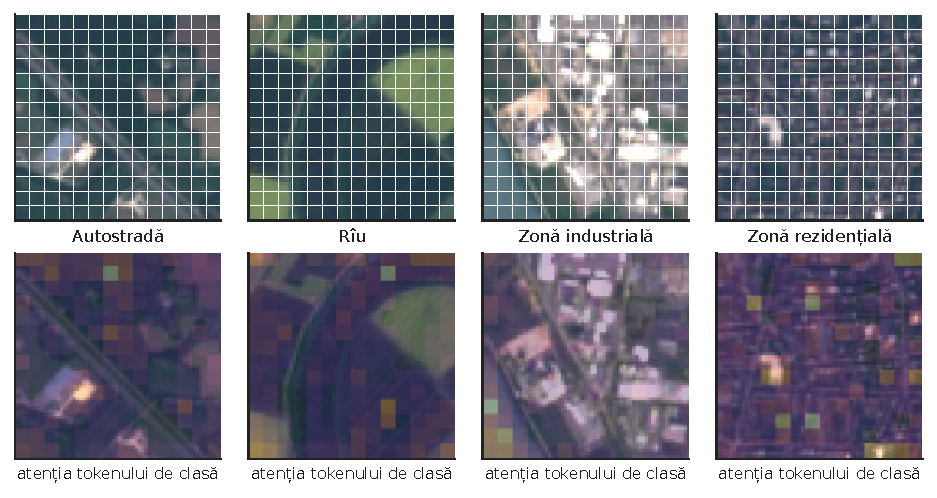
\includegraphics[width=\textwidth,height=0.519\textheight,keepaspectratio]{charts/ro/vit_patches_attention.pdf}\end{center}\vspace{-3mm}
\chartsource{Sursa: EuroSAT, imagini Sentinel-2 (Helber et al., 2019). Date: 4 imagini de test mărite la 224 x 224 de pixeli = 14 x 14 petice de 16 x 16; modelul CLIP ViT-B/16.}
\vspace{0.5mm}
\begin{itemize}\setlength{\itemsep}{0pt}
  \item Propagarea atenției: $\tilde{\mathbf A}=\prod_{\ell}(\frac12\bar{\mathbf A}_\ell+\frac12\mathbf I)$, rîndul tokenului de clasă
    \begin{itemize}\setlength{\itemsep}{0pt}
      \item $\bar{\mathbf A}_\ell$ = atenția stratului $\ell$, mediată pe capete.
    \end{itemize}
\end{itemize}
\par\vfill\noindent{\scriptsize\color{FooterGray}(Abnar \& Zuidema, 2020)}\hfill\qlink{NN\_L14\_vit\_patches\_attention}{Quantlets/L14/NN_L14_vit_patches_attention}\par\vspace{0.5mm}
\end{frame}


\section{CLIP: imagini și text în același spațiu}

\begin{frame}{CLIP învață potrivind imaginile cu descrierile lor}
\footnotesize
\intuition{într-un lot de $n$ perechi imagine--descriere, fiecare imagine își caută descrierea, și invers.}
\begin{columns}[T,onlytextwidth]
\begin{column}{0.58\textwidth}
\[ s_{ij}=\frac{\mathbf u_i^{\top}\mathbf v_j}{\tau},\quad \mathbf u_i=\frac{f(I_i)}{\lVert f(I_i)\rVert},\ \mathbf v_j=\frac{g(T_j)}{\lVert g(T_j)\rVert} \]\[ \loss=-\frac{1}{2n}\sum_{i=1}^{n}\Big[\log\frac{e^{s_{ii}}}{\sum_{j}e^{s_{ij}}}+\log\frac{e^{s_{ii}}}{\sum_{j}e^{s_{ji}}}\Big] \]{\footnotesize\begin{itemize}\setlength{\itemsep}{0pt}
  \item \textbf{\txtwhere}
    \begin{itemize}\setlength{\itemsep}{0pt}
      \item $f$ = codificatorul de imagini (ViT)
      \item $g$ = codificatorul de text
      \item $\tau$ = temperatura învățată
      \item Pierderea contrastivă (InfoNCE), în ambele direcții.
    \end{itemize}
\end{itemize}\par}
\end{column}
\begin{column}{0.39\textwidth}
\begin{itemize}\setlength{\itemsep}{2pt}
  \item \textbf{ViT-B/32}: 151{,}3 milioane de parametri
    \begin{itemize}\setlength{\itemsep}{0pt}
      \item \textbf{ViT-B/16}: 149{,}6 milioane.
    \end{itemize}
  \item \textbf{Nicio etichetă de clasă} nu a fost folosită la antrenare: doar descrieri de pe internet.
\end{itemize}
\end{column}
\end{columns}
\par\vfill\manager{un singur spațiu de embedding pentru imagini și text permite căutarea, etichetarea zero-shot și regăsirea pentru generarea augmentată prin regăsire (RAG).}\par\vspace{0.5mm}
\par\vfill\noindent{\scriptsize\color{FooterGray}(Radford et al., 2021; Oord et al., 2018)}\par\vspace{0.5mm}
\end{frame}

\begin{frame}{Clasificarea zero-shot: numele claselor devin clasificatorul}
\footnotesize
\intuition{se calculează embedding-ul unei propoziții pentru fiecare clasă și al imaginii, apoi se alege propoziția cea mai apropiată.}
\begin{columns}[T,onlytextwidth]
\begin{column}{0.53\textwidth}
\[ \mathbf w_c=\mathrm{norm}\Big(\frac{1}{M}\sum_{m=1}^{M}g\big(\text{template}_m(c)\big)\Big) \]\[ \hat c(I)=\argmax_c\ \mathbf u(I)^{\top}\mathbf w_c \]{\footnotesize\begin{itemize}\setlength{\itemsep}{0pt}
  \item \textbf{\txtwhere}
    \begin{itemize}\setlength{\itemsep}{0pt}
      \item Template$_m$ = o propoziție ca „a satellite photo of \{class\}.”
      \item $M$ = 1 sau 5 șabloane (ansamblu de prompturi)
      \item Descrierile claselor ca la Radford et al.\ (2021).
    \end{itemize}
\end{itemize}\par}
\end{column}
\begin{column}{0.44\textwidth}
\begin{itemize}\setlength{\itemsep}{2pt}
  \item \textbf{Cel mai bun zero-shot}: CLIP ViT-B/16, 56{,}4\,\% pe 5\,400 de imagini de test, fără niciun exemplu etichetat.
  \item \textbf{Nivelul hazardului} cu 10 clase: 10\,\%.
\end{itemize}
\end{column}
\end{columns}
\par\vfill\manager{vectorii de ponderi sînt scriși în limba engleză, deci un expert al domeniului poate modifica clasificatorul fără reantrenare.}\par\vspace{0.5mm}
\par\vfill\noindent{\scriptsize\color{FooterGray}(Radford et al., 2021)}\hfill\tryit{notebook \S2}\par\vspace{0.5mm}
\end{frame}

\begin{frame}{Cuvintele din prompt schimbă acuratețea zero-shot}
\small
\intuition{a-i spune lui CLIP că imaginea este o fotografie satelitară valorează mai mult decît un model mai mare.}
\begin{center}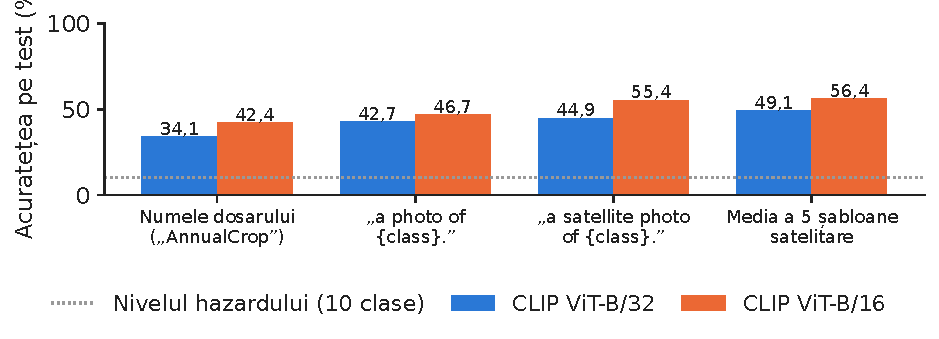
\includegraphics[width=\textwidth,height=0.428\textheight,keepaspectratio]{charts/ro/zeroshot_prompts.pdf}\end{center}\vspace{-3mm}
\chartsource{Sursa: EuroSAT, imagini Sentinel-2 (Helber et al., 2019). Date: 5400 de imagini de test, fără antrenare.}
\vspace{0.5mm}
\begin{itemize}\setlength{\itemsep}{0pt}
  \item ViT-B/16: numele dosarului 42{,}4\,\%, „a satellite photo of” 55{,}4\,\%, ansamblul de 5 șabloane 56{,}4\,\%
    \begin{itemize}\setlength{\itemsep}{0pt}
      \item ViT-B/32 ansamblu 49{,}1\,\%.
    \end{itemize}
\end{itemize}
\par\vfill\manager{formularea promptului este un hiperparametru: alegeți-o pe imagini de validare, apoi fixați-o.}\par\vspace{0.5mm}
\par\vfill\noindent{\scriptsize\color{FooterGray}}\hfill\qlink{NN\_L14\_zeroshot\_prompts}{Quantlets/L14/NN_L14_zeroshot_prompts}\par\vspace{0.5mm}
\end{frame}

\begin{frame}{Predicțiile zero-shot pe opt imagini de test alese aleator}
\small
\intuition{verde: corect; roșu: greșit; procentul este probabilitatea softmax a clasei alese.}
\begin{center}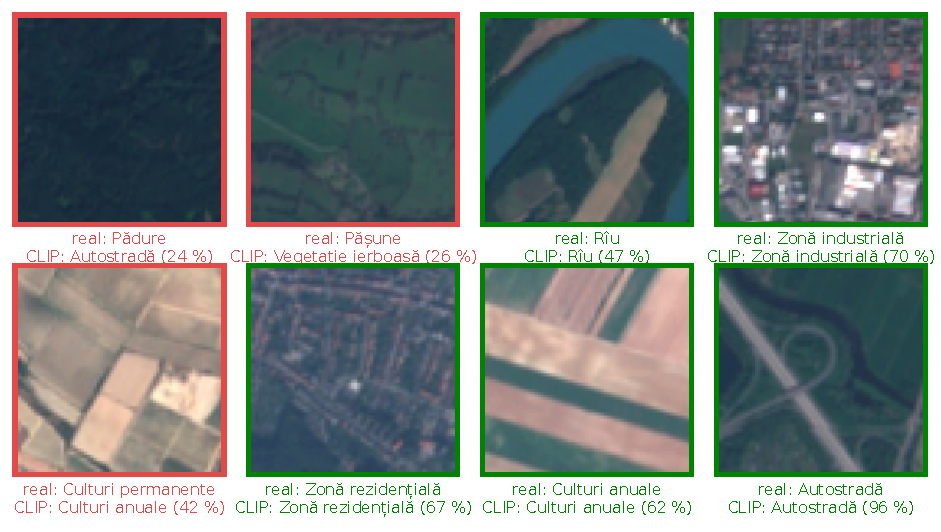
\includegraphics[width=\textwidth,height=0.567\textheight,keepaspectratio]{charts/ro/zeroshot_examples.pdf}\end{center}\vspace{-3mm}
\chartsource{Sursa: EuroSAT, imagini Sentinel-2 (Helber et al., 2019). Date: 8 imagini de test alese aleator (valoare fixă); verde = corect, roșu = greșit.}
\vspace{0.5mm}
\begin{itemize}\setlength{\itemsep}{0pt}
  \item 5 din 8 corecte în acest eșantion.
\end{itemize}
\par\vfill\noindent{\scriptsize\color{FooterGray}}\hfill\qlink{NN\_L14\_zeroshot\_examples}{Quantlets/L14/NN_L14_zeroshot_examples}\par\vspace{0.5mm}
\end{frame}

\begin{frame}{Unde greșește zero-shot: utilizări ale terenului care arată la fel}
\small
\intuition{rîndurile: clasa reală; coloanele: clasa prezisă; fiecare rînd însumează 100\,\%.}
\begin{center}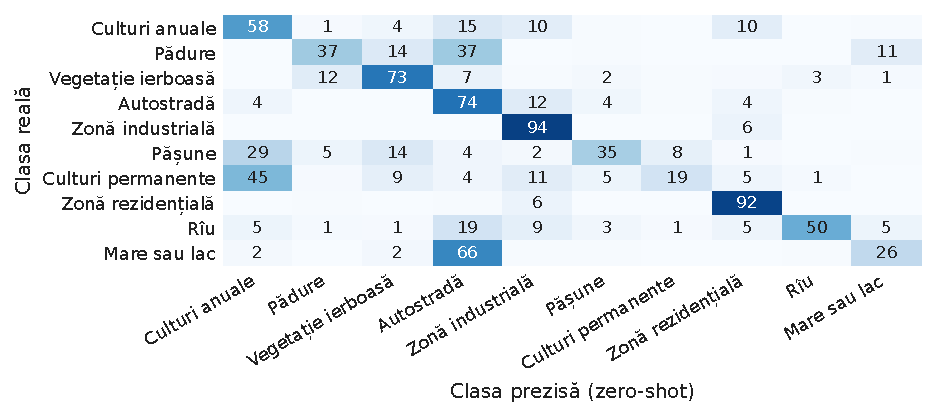
\includegraphics[width=\textwidth,height=0.524\textheight,keepaspectratio]{charts/ro/zeroshot_confusion.pdf}\end{center}\vspace{-3mm}
\chartsource{Sursa: EuroSAT, imagini Sentinel-2 (Helber et al., 2019). Date: 5400 de imagini de test; procente pe rînd.}
\vspace{0.5mm}
\begin{itemize}\setlength{\itemsep}{0pt}
  \item Cea mai bună clasă: zonă industrială (93{,}6\,\%)
    \begin{itemize}\setlength{\itemsep}{0pt}
      \item Cea mai slabă: culturi permanente (18{,}6\,\%)
      \item Cea mai mare confuzie: 399 din 600 imagini „mare sau lac” clasificate drept „autostradă”.
    \end{itemize}
\end{itemize}
\par\vfill\noindent{\scriptsize\color{FooterGray}}\hfill\qlink{NN\_L14\_zeroshot\_confusion}{Quantlets/L14/NN_L14_zeroshot_confusion}\par\vspace{0.5mm}
\end{frame}

\begin{frame}{Căutarea imaginilor cu ajutorul cuvintelor: aceleași embedding-uri, folosite invers}
\small
\intuition{ordonăm toate imaginile de test după similaritatea cu o propoziție; o bancă poate găsi terenuri inundate sau clădiri noi fără etichete.}
\vspace{-1mm}\[ \mathrm{P@}k(c)=\frac{1}{k}\sum_{j\in\mathrm{top}_k(\mathbf w_c)}\mathbb 1\{y_j=c\},\quad \mathrm{top}_k(\mathbf w_c)=\text{cele $k$ imagini cu cel mai mare}\ \mathbf u(I_j)^{\top}\mathbf w_c \]\vspace{-2mm}
\begin{center}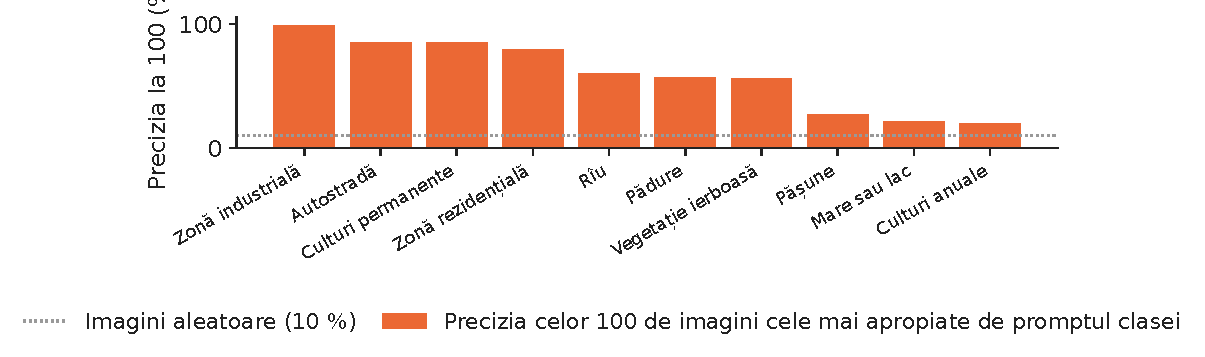
\includegraphics[width=\textwidth,height=0.210\textheight,keepaspectratio]{charts/ro/text_search.pdf}\end{center}\vspace{-3mm}
\chartsource{Sursa: EuroSAT, imagini Sentinel-2 (Helber et al., 2019). Date: 5400 de imagini de test; modelul CLIP ViT-B/16, 5 șabloane.}
\vspace{0.5mm}
\begin{itemize}\setlength{\itemsep}{0pt}
  \item Precizia medie a primelor 100: 58{,}9\,\%
    \begin{itemize}\setlength{\itemsep}{0pt}
      \item Cea mai bună: zonă industrială (99{,}0\,\%), cea mai slabă: culturi anuale (20{,}0\,\%).
    \end{itemize}
\end{itemize}
\par\vfill\manager{căutați întîi, etichetați rezultatele, apoi antrenați un clasificator: cea mai ieftină cale spre un set de imagini etichetate.}\par\vspace{0.5mm}
\par\vfill\noindent{\scriptsize\color{FooterGray}}\hfill\qlink{NN\_L14\_text\_search}{Quantlets/L14/NN_L14_text_search}\par\vspace{0.5mm}
\end{frame}

\begin{frame}{Un clasificator liniar pe trăsăturile CLIP: embedding plus regresie logistică}
\footnotesize
\intuition{CLIP rămîne fix și se antrenează doar o regresie logistică pe embedding-urile imaginilor.}
\begin{columns}[T,onlytextwidth]
\begin{column}{0.53\textwidth}
\[ \hat p(c\mid I)=\softmax\big(\mathbf W\mathbf u(I)+\mathbf b\big)_c \]\[ \min_{\mathbf W,\mathbf b}\ -\sum_{i}\log\hat p(c_i\mid I_i)+\frac{1}{2C}\lVert\mathbf W\rVert_F^2 \]{\footnotesize\begin{itemize}\setlength{\itemsep}{0pt}
  \item \textbf{\txtwhere}
    \begin{itemize}\setlength{\itemsep}{0pt}
      \item $\mathbf u(I)$ = embedding-ul normalizat ViT-B/16 (512 de dimensiuni)
      \item $C=10$, fixat a priori
      \item $k$ imagini etichetate pe clasă, 5 rulări.
    \end{itemize}
\end{itemize}\par}
\end{column}
\begin{column}{0.44\textwidth}
\begin{itemize}\setlength{\itemsep}{2pt}
  \item \textbf{Toate imaginile de antrenare}: 95{,}5\,\% (ViT-B/32: 94{,}8\,\%).
  \item \textbf{Depășește zero-shot} deja cu o singură imagine etichetată pe clasă: 59{,}0\,\%.
\end{itemize}
\end{column}
\end{columns}
\par\vfill\manager{un astfel de clasificator se antrenează în cîteva secunde pe laptop: primul lucru de încercat cînd aveți cîteva sute de etichete.}\par\vspace{0.5mm}
\par\vfill\noindent{\scriptsize\color{FooterGray}}\hfill\tryit{notebook \S3}\par\vspace{0.5mm}
\end{frame}

\begin{frame}{Trăsăturile preantrenate cîștigă cu puține etichete; o CNN antrenată cîștigă cu multe}
\small
\intuition{o imagine etichetată pe clasă depășește deja zero-shot; de la circa 64 pe clasă, o rețea mică antrenată de la zero o ajunge din urmă.}
\begin{center}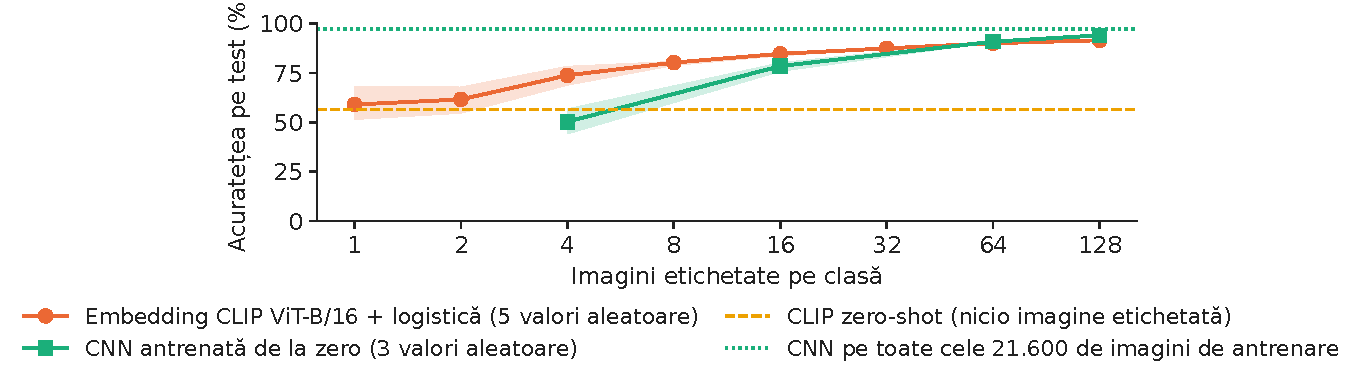
\includegraphics[width=\textwidth,height=0.206\textheight,keepaspectratio]{charts/ro/fewshot_eurosat.pdf}\end{center}\vspace{-3mm}
\chartsource{Sursa: EuroSAT, imagini Sentinel-2 (Helber et al., 2019). Date: 5400 de imagini de test; zona colorată = intervalul pe valorile generatorului aleator.}
\vspace{0.5mm}
\begin{itemize}\setlength{\itemsep}{0pt}
  \item 16 imagini pe clasă: clasificatorul pe embedding 84{,}7\,\%, CNN 78{,}5\,\%
    \begin{itemize}\setlength{\itemsep}{0pt}
      \item 128 pe clasă: 91{,}6\,\% față de 94{,}1\,\%
      \item Toate cele 21\,600 de imagini: CNN 97{,}4\,\%, clasificatorul pe embedding 95{,}5\,\%.
    \end{itemize}
\end{itemize}
\par\vfill\manager{cu multe etichete, o CNN mică recuperează
    \begin{itemize}\setlength{\itemsep}{0pt}
      \item Cu puține etichete, porniți de la un model fundație.
    \end{itemize}}\par\vspace{0.5mm}
\par\vfill\noindent{\scriptsize\color{FooterGray}}\hfill\qlink{NN\_L14\_fewshot\_eurosat}{Quantlets/L14/NN_L14_fewshot_eurosat}\par\vspace{0.5mm}
\end{frame}

\begin{frame}{Dimensiunea și viteza celor trei modele de imagini}
\small
{\footnotesize\renewcommand{\arraystretch}{1.05}\setlength{\tabcolsep}{4pt}
\begin{tabular}{@{}lrrr@{}}\toprule
Model & Parametri & ms pe imagine & Acuratețea pe test (\%) \\ \midrule
CNN de la zero (toate etichetele) & 289{,}2 mii & -- & 97{,}4 \\
CLIP ViT-B/32 + clasificator & 151{,}3 mil. & 4{,}23 & 94{,}8 \\
CLIP ViT-B/16 + clasificator & 149{,}6 mil. & 20{,}49 & 95{,}5 \\
Qwen2-VL-2B (întrebări despre grafice) & 2{,}21 mld. & 262 & -- \\
\bottomrule\end{tabular}}
\par\vspace{0.5mm}{\scriptsize \begin{itemize}\setlength{\itemsep}{0pt}
  \item Timp măsurat pe un laptop (procesor grafic Apple silicon), pentru calculul embedding-ului unei imagini în loturi; timpul VLM include întrebarea.
  \item Un petic mai mare (32 de pixeli în loc de 16) înseamnă de 4 ori mai puțini tokeni: mai rapid, puțin mai puțin precis.
\end{itemize}}
\par\vfill\noindent{\scriptsize\color{FooterGray}(calcul propriu)}\par\vspace{0.5mm}
\end{frame}


\section{Modele vizual-lingvistice: citirea graficelor și a tabelelor}

\begin{frame}{Un VLM conectează un codificator de imagini la un model de limbaj}
\footnotesize
\intuition{peticele imaginii sînt proiectate în spațiul embedding-urilor de cuvinte al unui model lingvistic mare (LLM), care le citește ca tokeni suplimentari.}
\begin{columns}[T,onlytextwidth]
\begin{column}{0.53\textwidth}
\[ \mathbf H_v=\mathbf W_p\,f_{\text{ViT}}(I) \]\[ p(y_t\mid y_{<t},I,q)=\mathrm{LLM}_{\btheta}\big([\mathbf H_v;\ \mathbf e(q);\ \mathbf e(y_{<t})]\big) \]{\footnotesize\begin{itemize}\setlength{\itemsep}{0pt}
  \item \textbf{\txtwhere}
    \begin{itemize}\setlength{\itemsep}{0pt}
      \item $f_{\text{ViT}}$ = codificatorul vizual
      \item $\mathbf W_p$ = proiectorul (un MLP)
      \item $q$ = întrebarea
      \item Antrenat întîi pe perechi imagine--descriere, apoi pe instrucțiuni vizuale.
    \end{itemize}
\end{itemize}\par}
\end{column}
\begin{column}{0.44\textwidth}
\begin{itemize}\setlength{\itemsep}{2pt}
  \item \textbf{Asistentul lingvistic și vizual (LLaVA)} a introdus această rețetă
    \begin{itemize}\setlength{\itemsep}{0pt}
      \item Qwen2-VL adaugă imagini de orice rezoluție.
    \end{itemize}
  \item \textbf{Modelul nostru}: Qwen2-VL-2B-Instruct, 2{,}21 miliarde de parametri, rulat local.
\end{itemize}
\end{column}
\end{columns}
\par\vfill\manager{răspunsul este text generat: restrîngeți-l (da/nu, un număr) și evaluați-l ca pe un clasificator.}\par\vspace{0.5mm}
\par\vfill\noindent{\scriptsize\color{FooterGray}(Liu et al., 2023; Wang et al., 2024)}\par\vspace{0.5mm}
\end{frame}

\begin{frame}{Regimurile pieței ca problemă de recunoaștere vizuală}
\footnotesize
\intuition{desenăm ultimele 120 de zile ale S\&P 500 ca imagine și întrebăm dacă piața este în criză, cum ar face un analist tehnic.}
\begin{columns}[T,onlytextwidth]
\begin{column}{0.53\textwidth}
\[ S_t=\mathbb 1\Big\{\sigma^{(20)}_t>Q_{0.9}\big(\sigma^{(20)}_{t-750:t-1}\big)\Big\} \]\[ \sigma^{(20)}_t=\sqrt{252}\,\mathrm{sd}(r_{t-19:t}) \]{\footnotesize\begin{itemize}\setlength{\itemsep}{0pt}
  \item \textbf{\txtwhere}
    \begin{itemize}\setlength{\itemsep}{0pt}
      \item $S_t$ = eticheta de criză la sfîrșitul ferestrei: volatilitatea pe 20 de zile peste percentila 90 glisantă din ultimii trei ani (doar date din trecut)
      \item Ferestre la fiecare 5 zile
      \item Antrenare pînă în 2018, test pe 394 de ferestre din 2019.
    \end{itemize}
\end{itemize}\par}
\end{column}
\begin{column}{0.44\textwidth}
\begin{itemize}\setlength{\itemsep}{2pt}
  \item \textbf{Patru metode pe aceleași ferestre}
    \begin{itemize}\setlength{\itemsep}{0pt}
      \item Cifre + regresie logistică (randamente, volatilitate, scădere de la maxim)
      \item Embedding-ul CLIP al imaginii + regresie logistică
      \item CLIP zero-shot: „calm, în creștere constantă” față de „volatil, prăbușire bruscă”
      \item Qwen2-VL zero-shot: „este piața agitată?” da sau nu
    \end{itemize}
\end{itemize}
\end{column}
\end{columns}
\par\vfill\manager{o etichetă bazată pe cuantile glisante evită etichetarea manuală și folosirea viitorului.}\par\vspace{0.5mm}
\par\vfill\noindent{\scriptsize\color{FooterGray}(Jheng, Pele, Tak \& Găman, 2026)}\hfill\tryit{notebook \S4}\par\vspace{0.5mm}
\end{frame}

\begin{frame}{Din imagine sau din cifre? Detectarea crizelor de piață}
\small
\intuition{stînga: o fereastră calmă și una de criză, așa cum le văd modelele; dreapta: curbele caracteristicii de operare a receptorului (ROC) pe anii de test.}
\begin{center}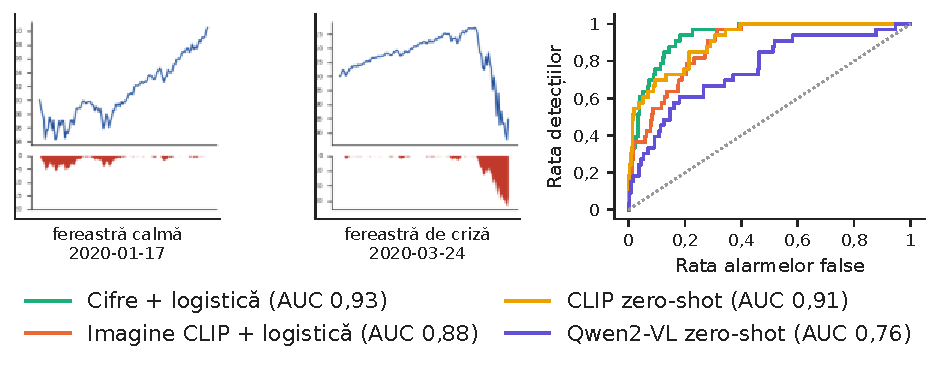
\includegraphics[width=\textwidth,height=0.434\textheight,keepaspectratio]{charts/ro/chart_regime.pdf}\end{center}\vspace{-3mm}
\chartsource{Sursa: Yahoo Finance, cotații zilnice. Date: S\&P 500, ferestre de 120 de zile de tranzacționare la fiecare 5 zile; test 7 ianuarie 2019 - 30 octombrie 2026.}
\vspace{0.5mm}
\begin{itemize}\setlength{\itemsep}{0pt}
  \item Aria de sub curba ROC (AUC): cifre 0{,}933, clasificator pe CLIP 0{,}880, CLIP zero-shot 0{,}907, Qwen2-VL zero-shot 0{,}758
    \begin{itemize}\setlength{\itemsep}{0pt}
      \item Ponderea crizelor în test 8{,}4\,\%.
    \end{itemize}
\end{itemize}
\par\vfill\noindent{\scriptsize\color{FooterGray}}\hfill\qlink{NN\_L14\_chart\_regime}{Quantlets/L14/NN_L14_chart_regime}\par\vspace{0.5mm}
\end{frame}

\begin{frame}{Detectarea crizelor: capacitatea de separare și precizia pe anii de test}
\small
\begin{columns}[T,onlytextwidth]
\begin{column}{0.5\textwidth}
{\scriptsize\renewcommand{\arraystretch}{1.05}\setlength{\tabcolsep}{4pt}
\begin{tabular}{@{}lrrl@{}}\toprule
Metoda & AUC & Prec.\ medie & Etichete \\ \midrule
Cifre + logistică & \cellcolor{Forest!55}0{,}933 & \cellcolor{Forest!49}0{,}578 & da \\
Imagine CLIP + logistică & \cellcolor{Forest!42}0{,}880 & \cellcolor{Forest!22}0{,}449 & da \\
CLIP zero-shot & \cellcolor{Forest!48}0{,}907 & \cellcolor{Forest!55}0{,}605 & nu \\
Qwen2-VL zero-shot & \cellcolor{Forest!11}0{,}758 & \cellcolor{Crimson!9}0{,}302 & nu \\
\bottomrule\end{tabular}}
\end{column}
\begin{column}{0.47\textwidth}
\begin{itemize}\setlength{\itemsep}{4pt}
  \item \textbf{Cel mai bun}: cifrele.
  \item \textbf{Precizia medie} a unui scor aleator = ponderea crizelor, 8{,}4\,\%.
  \item \textbf{Lecția}: cînd cifrele există, imaginea adaugă un pas cu pierdere de informație
    \begin{itemize}\setlength{\itemsep}{0pt}
      \item Imaginile își au locul cînd cifrele lipsesc (scanări, capturi de ecran, imagini satelitare).
    \end{itemize}
\end{itemize}
\end{column}
\end{columns}
\par\vfill\noindent{\scriptsize\color{FooterGray}(calcul propriu, după Jheng, Pele, Tak \& Găman, 2026)}\hfill\tryit{notebook \S4}\par\vspace{0.5mm}
\end{frame}

\begin{frame}{Ce poate citi un VLM de 2 miliarde de parametri: tendințe și celule de tabel}
\small
\begin{itemize}\setlength{\itemsep}{3pt}
  \item \textbf{Întrebarea despre tendință}, pe 394 de grafice de test: „prețul a încheiat mai sus sau mai jos?”
    \begin{itemize}\setlength{\itemsep}{0pt}
      \item Acuratețe 57{,}1\,\% la pragul de 0,5, sub răspunsul constant cu clasa majoritară (74{,}9\,\%)
      \item Totuși AUC 0{,}974: ordonarea este corectă, pragul este deplasat --- recalibrați pe grafice de validare
    \end{itemize}
  \item \textbf{Întrebarea despre tabel}, pe 60 de tabele ale curbei randamentelor BCE: „care este randamentul la 10 ani?”
    \begin{itemize}\setlength{\itemsep}{0pt}
      \item Răspunsuri exacte 25{,}0\,\%; eroarea absolută medie 0{,}192 puncte procentuale; numere extrase 100{,}0\,\%
    \end{itemize}
  \item \textbf{De ce contează}
    \begin{itemize}\setlength{\itemsep}{0pt}
      \item Citirea unei celule înseamnă recunoaștere optică a caracterelor (OCR) plus găsirea coloanei: erorile sînt tăcute și plauzibile
      \item Pentru documente cu structură cunoscută, extrageți cifrele cu un program de citire și folosiți VLM doar unde structura variază
    \end{itemize}
\end{itemize}
\par\vfill\noindent{\scriptsize\color{FooterGray}(calcul propriu; Wang et al., 2024)}\hfill\tryit{notebook \S5}\par\vspace{0.5mm}
\end{frame}

\begin{frame}{Fluxul documentelor într-o bancă: unde se potrivește un VLM}
\small
\begin{itemize}\setlength{\itemsep}{3pt}
  \item \textbf{1. Preluarea}
    \begin{itemize}\setlength{\itemsep}{0pt}
      \item Pagină scanată sau fișier electronic; șabloanele cunoscute merg la un program de citire bazat pe reguli
    \end{itemize}
  \item \textbf{2. Citirea}
    \begin{itemize}\setlength{\itemsep}{0pt}
      \item OCR și așezarea în pagină pentru text și tabele; un VLM pentru pagini libere, grafice și ștampile
    \end{itemize}
  \item \textbf{3. Verificarea}
    \begin{itemize}\setlength{\itemsep}{0pt}
      \item Totalurile trebuie să se adune, datele să fie valide, valorile în intervale plauzibile; o verificare eșuată merge la un om
    \end{itemize}
  \item \textbf{4. Măsurarea}
    \begin{itemize}\setlength{\itemsep}{0pt}
      \item Rata de potrivire exactă pe fiecare cîmp, pe un eșantion etichetat, ca la tabelele de randamente (aici 25{,}0\,\%)
    \end{itemize}
\end{itemize}
\end{frame}

\begin{frame}{Ce pot și ce nu pot (încă) face modelele multimodale}
\small
\begin{columns}[T,onlytextwidth]
\begin{column}{0.49\textwidth}
\begin{itemize}\setlength{\itemsep}{3pt}
  \item \textbf{Pot}
    \begin{itemize}\setlength{\itemsep}{0pt}
      \item Eticheta imagini fără date de antrenare (56{,}4\,\% pe EuroSAT)
      \item Oferi trăsături care au nevoie de puține etichete (84{,}7\,\% cu 16 pe clasă)
      \item Căuta imagini după text și text după imagini
      \item Răspunde la întrebări simple despre grafice și documente
    \end{itemize}
\end{itemize}
\end{column}
\begin{column}{0.48\textwidth}
\begin{itemize}\setlength{\itemsep}{3pt}
  \item \textbf{Nu pot (în mod fiabil)}
    \begin{itemize}\setlength{\itemsep}{0pt}
      \item Înlocui cifrele din spatele unui grafic
      \item Citi corect fiecare celulă a unui tabel (aici, 25{,}0\,\% exact)
      \item Explica fidel de ce au răspuns astfel
      \item Separa fără exemple clasele care arată la fel
    \end{itemize}
\end{itemize}
\end{column}
\end{columns}
\par\vspace{0.5mm}{\scriptsize \begin{itemize}\setlength{\itemsep}{0pt}
  \item Măsuri de control: un set de test etichetat, răspunsuri restrînse, verificarea umană a cazurilor cu încredere scăzută, jurnalizarea fiecărui prompt și a fiecărei imagini.
\end{itemize}}
\end{frame}


\section{Sinteza cursului}

\begin{frame}{Paisprezece cursuri, o singură trusă de instrumente}
\small
{\scriptsize\renewcommand{\arraystretch}{1.05}\setlength{\tabcolsep}{4pt}
\begin{tabular}{@{}p{0.2\textwidth}p{0.36\textwidth}p{0.37\textwidth}@{}}\toprule
Date & Modele & Cursuri și aplicații \\ \midrule
Tabele & regresie logistică, MLP, regularizare & 1--3: scoring de credit, fraudă \\
Imagini & CNN, transferul învățării, ViT, CLIP & 4, 14: utilizarea terenului, documente \\
Secvențe & rețele cu memorie pe termen scurt și lung (LSTM), rețele cu expansiune în baze, modele fundație & 5, 13: prețuri, consum, valoarea expusă la risc (VaR) \\
Text & embedding, transformere, LLM, generare augmentată prin regăsire (RAG) & 6, 7, 12: sentiment, bănci centrale \\
Generare & autoencoder variațional (VAE), rețea generativă adversarială (GAN), difuzie & 8: date sintetice, anomalii \\
Grafuri & rețea neuronală pe grafuri (GNN) & 9: rețele de tranzacții \\
Decizii & învățare prin recompensă (RL) & 10: tranzacționare, acoperirea riscului, baterii \\
Încredere & inteligență artificială explicabilă (XAI): explicații aditive Shapley (SHAP), gradienți & 11: auditul modelelor de credit \\
\bottomrule\end{tabular}}
\end{frame}

\begin{frame}{Alegerea modelului pentru o problemă de afaceri}
\small
\begin{itemize}\setlength{\itemsep}{2pt}
  \item \textbf{1. Porniți de la decizie și de la costul erorilor}
    \begin{itemize}\setlength{\itemsep}{0pt}
      \item O fraudă ratată și o alarmă falsă nu costă la fel; alegeți metrica înaintea modelului
    \end{itemize}
  \item \textbf{2. Estimați întîi reperul}
    \begin{itemize}\setlength{\itemsep}{0pt}
      \item Regresie logistică, prognoza naivă, o autoregresie Lasso, un model de volatilitate, frecvențe de cuvinte cu un clasificator liniar: cîteva minute, ușor de interpretat
    \end{itemize}
  \item \textbf{3. Numărați etichetele}
    \begin{itemize}\setlength{\itemsep}{0pt}
      \item Puține etichete: model fundație zero-shot sau cu un clasificator pe embedding; multe etichete: o rețea antrenată
    \end{itemize}
  \item \textbf{4. Potriviți arhitectura cu datele}
    \begin{itemize}\setlength{\itemsep}{0pt}
      \item Tabele: MLP sau boosting; imagini: CNN sau ViT; secvențe: rețele recurente sau transformer; grafuri: GNN
    \end{itemize}
  \item \textbf{5. Demonstrați}
    \begin{itemize}\setlength{\itemsep}{0pt}
      \item Testare o singură dată, mai multe rulări, un test de semnificație, calibrare, o explicație pentru autoritatea de supraveghere
    \end{itemize}
\end{itemize}
\end{frame}

\begin{frame}{Cinci reguli de evaluare valabile în fiecare curs}
\small
\begin{itemize}\setlength{\itemsep}{4pt}
  \item \textbf{Fără scurgeri de informație}: scalările, prompturile și pragurile se aleg pe datele de antrenare sau de validare
    \begin{itemize}\setlength{\itemsep}{0pt}
      \item Seriile de timp se împart cronologic.
    \end{itemize}
  \item \textbf{Un reper lîngă fiecare rețea}: aici, o CNN antrenată de la zero lîngă CLIP, cifrele lîngă imaginile graficelor.
  \item \textbf{Rulări repetate și intervale}: rezultatele cu puține exemple de mai sus sînt medii pe 5 rulări, cu amplitudinea lor.
  \item \textbf{Metrici pentru evenimente rare}: precizia medie și AUC pentru crize, nu acuratețea.
  \item \textbf{Date reale, rezultate reproductibile}: fiecare cifră provine dintr-un program și dintr-un set de date public, cu un Quantlet.
\end{itemize}
\end{frame}

\begin{frame}{Modelele fundație în acest curs: un singur tipar, trei tipuri de date}
\small
\begin{itemize}\setlength{\itemsep}{3pt}
  \item \textbf{Tiparul}
    \begin{itemize}\setlength{\itemsep}{0pt}
      \item Preantrenare o singură dată pe volume uriașe de date neetichetate; utilizare zero-shot, cu cîteva exemple sau cu un mic clasificator antrenat
    \end{itemize}
  \item \textbf{Text} (cursul 12)
    \begin{itemize}\setlength{\itemsep}{0pt}
      \item Prompturi și embedding LLM pentru sentiment, RAG pe discursurile BCE, LLM-VaR
    \end{itemize}
  \item \textbf{Serii de timp} (cursul 13)
    \begin{itemize}\setlength{\itemsep}{0pt}
      \item Modele de tip Chronos prognozează prețuri, consum și VaR fără antrenare
    \end{itemize}
  \item \textbf{Imagini} (acest curs)
    \begin{itemize}\setlength{\itemsep}{0pt}
      \item CLIP zero-shot 56{,}4\,\%; clasificator pe toate etichetele 95{,}5\,\%
    \end{itemize}
  \item \textbf{Avertismentul comun}
    \begin{itemize}\setlength{\itemsep}{0pt}
      \item Datele de preantrenare pot conține setul dumneavoastră de test; evaluați pe date pe care modelul nu le-a putut vedea
    \end{itemize}
\end{itemize}
\end{frame}

\begin{frame}{Zece formule ale cursului (1/2): învățarea}
\small
{\footnotesize\renewcommand{\arraystretch}{1.4}\setlength{\tabcolsep}{4pt}
\begin{tabular}{@{}p{0.27\textwidth}p{0.47\textwidth}p{0.18\textwidth}@{}}\toprule
Idee & Formula & Cursul \\ \midrule
Neuronul logistic & $\hat p=\sigma(\mathbf w^{\top}\mathbf x+b)$ & 1 \\
Pierderea entropie încrucișată & $\loss=-\sum_i[y_i\log\hat p_i+(1-y_i)\log(1-\hat p_i)]$ & 1--2 \\
Propagarea înapoi & $\boldsymbol\delta^{(\ell)}=(\mathbf W^{(\ell+1)\top}\boldsymbol\delta^{(\ell+1)})\odot f'(\mathbf z^{(\ell)})$ & 2 \\
Pasul de gradient (Adam fără momente) & $\btheta\leftarrow\btheta-\eta\nabla_{\btheta}\loss$ & 2 \\
Penalizarea ponderilor & $\loss+\lambda\lVert\btheta\rVert_2^2$ & 3 \\
\bottomrule\end{tabular}}
\par\vspace{0.5mm}{\scriptsize \begin{itemize}\setlength{\itemsep}{0pt}
  \item Toate simbolurile, ca în cursurile citate; $\sigma$ = funcția logistică, $\odot$ = produsul element cu element.
\end{itemize}}
\end{frame}

\begin{frame}{Zece formule ale cursului (2/2): arhitecturi}
\small
{\footnotesize\renewcommand{\arraystretch}{1.4}\setlength{\tabcolsep}{4pt}
\begin{tabular}{@{}p{0.27\textwidth}p{0.47\textwidth}p{0.18\textwidth}@{}}\toprule
Idee & Formula & Cursul \\ \midrule
Convoluția & $(\mathbf K*\mathbf X)_{ij}=\sum_{u,v}K_{uv}X_{i+u,j+v}$ & 4 \\
Starea recurentă & $\mathbf h_t=\tanh(\mathbf W\mathbf h_{t-1}+\mathbf U\mathbf x_t+\mathbf b)$ & 5 \\
Atenția & $\softmax(\mathbf Q\mathbf K^{\top}/\sqrt{d_k})\mathbf V$ & 7, 12--14 \\
Convoluția pe graf & $\mathbf H'=\sigma(\tilde{\mathbf D}^{-1/2}\tilde{\mathbf A}\tilde{\mathbf D}^{-1/2}\mathbf H\mathbf W)$ & 9 \\
Pierderea contrastivă imagine--text & $-\log\frac{e^{s_{ii}}}{\sum_j e^{s_{ij}}}$ & 14 \\
\bottomrule\end{tabular}}
\par\vspace{0.5mm}{\scriptsize \begin{itemize}\setlength{\itemsep}{0pt}
  \item $\mathbf K$ = nucleul; $\tilde{\mathbf A}$ = matricea de adiacență cu bucle, $\tilde{\mathbf D}$ matricea gradelor; $s_{ij}$ = similaritatea scalată imagine--text.
\end{itemize}}
\end{frame}

\begin{frame}{Utilizarea responsabilă: aceleași reguli pentru fiecare model din curs}
\small
\begin{itemize}\setlength{\itemsep}{3pt}
  \item \textbf{Reglementare}
    \begin{itemize}\setlength{\itemsep}{0pt}
      \item Regulamentul UE privind inteligența artificială (2024/1689) include scoringul de credit printre utilizările cu risc ridicat: documentație, supraveghere umană, guvernanța datelor
    \end{itemize}
  \item \textbf{Documentare}
    \begin{itemize}\setlength{\itemsep}{0pt}
      \item O fișă a modelului: date, perioadă, metrică, reper, rulări, cazuri cunoscute de eșec (aici: mare sau lac citit drept autostradă)
    \end{itemize}
  \item \textbf{Monitorizare}
    \begin{itemize}\setlength{\itemsep}{0pt}
      \item Retestare pe date noi: regimuri de preț, noi sezoane satelitare, teme noi în discursuri
    \end{itemize}
  \item \textbf{Confidențialitate}
    \begin{itemize}\setlength{\itemsep}{0pt}
      \item Modelele deschise rulate local păstrează documentele și imaginile clienților în instituție
    \end{itemize}
\end{itemize}
\end{frame}

\begin{frame}{Cum arată un proiect bun pentru acest curs}
\small
\begin{columns}[T,onlytextwidth]
\begin{column}{0.49\textwidth}
\begin{itemize}\setlength{\itemsep}{3pt}
  \item \textbf{Întrebare și date}
    \begin{itemize}\setlength{\itemsep}{0pt}
      \item O decizie de afaceri, un set de date public, perioada și licența lui
    \end{itemize}
  \item \textbf{Întîi reperul}
    \begin{itemize}\setlength{\itemsep}{0pt}
      \item Un model liniar sau naiv, raportat lîngă fiecare rețea
    \end{itemize}
  \item \textbf{Verificarea scurgerilor}
    \begin{itemize}\setlength{\itemsep}{0pt}
      \item Împărțire în ordine cronologică, scalări estimate pe antrenare, testul folosit o singură dată
    \end{itemize}
\end{itemize}
\end{column}
\begin{column}{0.48\textwidth}
\begin{itemize}\setlength{\itemsep}{3pt}
  \item \textbf{Incertitudine}
    \begin{itemize}\setlength{\itemsep}{0pt}
      \item Mai multe rulări, intervale bootstrap sau un test Diebold--Mariano
    \end{itemize}
  \item \textbf{Explicație}
    \begin{itemize}\setlength{\itemsep}{0pt}
      \item SHAP sau gradienți pentru decizia care contează
    \end{itemize}
  \item \textbf{Reproductibil}
    \begin{itemize}\setlength{\itemsep}{0pt}
      \item Un singur program, de la datele brute la fiecare cifră și grafic
    \end{itemize}
\end{itemize}
\end{column}
\end{columns}
\end{frame}

\begin{frame}{Probleme deschise care merită o lucrare de disertație}
\small
\begin{columns}[T,onlytextwidth]
\begin{column}{0.49\textwidth}
\begin{itemize}\setlength{\itemsep}{4pt}
  \item \textbf{Calibrarea în prezența derivei}: benzi conformale care rămîn valide cînd piețele își schimbă regimul.
  \item \textbf{Evaluarea fără scurgeri de informație} a modelelor fundație antrenate pe internet.
  \item \textbf{Explicații stabile}: rezistă valorile SHAP ale unui model de credit la o reantrenare?
\end{itemize}
\end{column}
\begin{column}{0.48\textwidth}
\begin{itemize}\setlength{\itemsep}{4pt}
  \item \textbf{Modele mici pentru instituții mici}: cînd ajunge un model de 2--3 miliarde de parametri pe un laptop?
  \item \textbf{Semnale de risc multimodale}: imagini satelitare, text și prețuri într-un singur model de avertizare timpurie.
  \item \textbf{Date românești}: modele de limbaj și prognoze pentru textul, piețele și energia din România.
\end{itemize}
\end{column}
\end{columns}
\end{frame}

\section*{Recapitulare}

\begin{frame}{Test 1: clasificatorul zero-shot}
\small
\begin{itemize}
  \item O bancă vrea să marcheze terenurile inundate în imagini satelitare, dar nu are nicio imagine etichetată
    \begin{itemize}\setlength{\itemsep}{0pt}
      \item Ce poate face cu CLIP?
    \end{itemize}
\end{itemize}
\vspace{2mm}
\begin{exampleblock}{R\u{a}spuns}
\begin{itemize}
  \item Scrie prompturi pentru clase („a satellite photo of a flooded field”, „\ldots{} of a dry field”), le calculează embedding-urile și clasifică după similaritatea cosinus
    \begin{itemize}\setlength{\itemsep}{0pt}
      \item Apoi etichetează cîteva sute de imagini pentru validare și pentru un clasificator pe embedding.
    \end{itemize}
\end{itemize}
\end{exampleblock}
\end{frame}

\begin{frame}{Test 2: imagini sau cifre}
\small
\begin{itemize}
  \item De ce a detectat modelul logistic pe cifre crizele de piață cel puțin la fel de bine ca modelele care citesc imaginea graficului?
\end{itemize}
\vspace{2mm}
\begin{exampleblock}{R\u{a}spuns}
\begin{itemize}
  \item Imaginea este desenată din aceleași cifre, cu pierdere de rezoluție
    \begin{itemize}\setlength{\itemsep}{0pt}
      \item Cifrele conțin direct volatilitatea.
      \item Imaginile ajută cînd nu există cifre.
    \end{itemize}
\end{itemize}
\end{exampleblock}
\end{frame}

\begin{frame}{Test 3: etichetele}
\small
\begin{itemize}
  \item Cu 16 imagini etichetate pe clasă, ce alegeți: o CNN de la zero sau un clasificator pe embedding-urile CLIP?
\end{itemize}
\vspace{2mm}
\begin{exampleblock}{R\u{a}spuns}
\begin{itemize}
  \item Clasificatorul pe embedding: 84{,}7\,\%, față de 78{,}5\,\% pentru CNN, pe datele noastre.
\end{itemize}
\end{exampleblock}
\end{frame}

\begin{frame}{Recapitulare}
\small
\begin{itemize}\setlength{\itemsep}{4pt}
  \item Un ViT citește imaginile ca tokeni-petic
    \begin{itemize}\setlength{\itemsep}{0pt}
      \item CLIP le aliniază cu textul printr-o pierdere contrastivă.
    \end{itemize}
  \item CLIP zero-shot etichetează imaginile satelitare cu 56{,}4\,\%, fără etichete
    \begin{itemize}\setlength{\itemsep}{0pt}
      \item Un clasificator pe embedding ajunge la 95{,}5\,\%.
    \end{itemize}
  \item Modelele VLM răspund la întrebări despre grafice și tabele, dar trebuie evaluate ca orice clasificator.
  \item Cursul într-un rînd: întîi reperul, date reale, fără scurgeri de informație, mai multe rulări, un test, o explicație.
\end{itemize}
\end{frame}

\begin{frame}{Cercetările grupului nostru}
\footnotesize
\begin{itemize}\setlength{\itemsep}{3pt}
  \item \textbf{Detectarea anomaliilor cu modele vizual-lingvistice} (premiul pentru cea mai bună lucrare, Conferința internațională Business Excellence (ICBE) 2026): indicatorii de piață sînt proiectați pe imagini cu mai multe panouri, iar un VLM (GPT-4.1, transformer generativ preantrenat) clasifică regimul zero-shot, cu etichete bazate pe cuantile glisante, și își explică alegerea
    \begin{itemize}\setlength{\itemsep}{0pt}
      \item Validare pe date noi pentru S\&P 500 (Jheng, Pele, Tak \& Găman, 2026, PICBE).
    \end{itemize}
  \item \textbf{Detectarea explicabilă a fraudei}: modele tabulare și rețele pe grafuri, combinate cu SHAP și ablația grafului (Diaconu \& Pele, 2026, PICBE) --- studiul de caz 1.
  \item \textbf{LLM-VaR și LLM-ES}: modelele de limbaj ca modele de risc zero-shot (Pele et al., 2026, Expert Systems with Applications) --- cursurile 12 și 13.
  \item \textbf{Portofolii care țin cont de ESG}: selecția activelor după mai multe criterii, cu scoruri ESG (Găman, Tak, Jheng \& Pele, 2026, PICBE).
\end{itemize}
\par\vspace{0.5mm}{\scriptsize \begin{itemize}\setlength{\itemsep}{0pt}
  \item Rezultatele sînt preluate din rezumatele lucrărilor; cifrele de pe celelalte slide-uri provin din datele noastre.
\end{itemize}}
\par\vfill\noindent{\scriptsize\color{FooterGray}(Academia de Studii Economice din București, ASE; Academia Română, Institutul de Prognoză Economică, IPE)}\par\vspace{0.5mm}
\end{frame}

\begin{frame}{Vreți să aflați mai mult?}
\small
\begin{columns}[T,onlytextwidth]
\begin{column}{0.5\textwidth}
\begin{itemize}\setlength{\itemsep}{4pt}
  \item \textbf{OpenCLIP}, modele și evaluări: \href{https://github.com/mlfoundations/open_clip}{github.com/mlfoundations/open\_clip}.
  \item \textbf{Qwen2-VL}: \href{https://github.com/QwenLM/Qwen2-VL}{github.com/QwenLM/Qwen2-VL}.
  \item \textbf{Bishop \& Bishop (2024)}, capitolele 12 și 20: \href{https://www.bishopbook.com}{bishopbook.com}.
\end{itemize}
\end{column}
\begin{column}{0.47\textwidth}
\begin{itemize}\setlength{\itemsep}{4pt}
  \item \textbf{Quantinar}: Digital Transformation on Finance: \href{https://quantinar.com/course/674/digital-transformation-on-finance}{quantinar.com}.
  \item \textbf{EuroSAT}, date: \href{https://github.com/phelber/EuroSAT}{github.com/phelber/EuroSAT}.
  \item \textbf{Acest curs}: notebook, seminar și Quantlets --- \href{https://github.com/danpele/NEURAL_BIZ}{github.com/danpele/NEURAL\_BIZ}.
\end{itemize}
\end{column}
\end{columns}
\end{frame}

\begin{frame}{Bibliografie (1/2)}
\scriptsize
\begin{itemize}\setlength{\itemsep}{0pt}\scriptsize
\item Abnar, S.\ \& Zuidema, W.\ (2020). Quantifying attention flow in transformers. \textit{Proceedings of the 58th Annual Meeting of the Association for Computational Linguistics}, 4190--4197. \href{https://doi.org/10.18653/v1/2020.acl-main.385}{doi:10.18653/v1/2020.acl-main.385}
\item Bishop, C.\,M.\ \& Bishop, H.\ (2024). \textit{Deep Learning: Foundations and Concepts}. Springer. \href{https://doi.org/10.1007/978-3-031-45468-4}{doi:10.1007/978-3-031-45468-4}
\item Diaconu, D.\ \& Pele, D.\,T.\ (2026). Explainable AI in financial fraud detection: Evidence from the IEEE-CIS fraud dataset. \textit{Proceedings of the International Conference on Business Excellence}, 20(1), 118--132. \href{https://doi.org/10.2478/picbe-2026-0015}{doi:10.2478/picbe-2026-0015}
\item Dosovitskiy, A.\ et al.\ (2021). An image is worth 16x16 words: Transformers for image recognition at scale. \textit{International Conference on Learning Representations}. \href{https://arxiv.org/abs/2010.11929}{arXiv:2010.11929}
\item Găman, Ș., Tak, R., Jheng, S.-L.\ \& Pele, D.\,T.\ (2026). ESG-aware asset selection and portfolio optimization: A comparative study of multi-criteria decision-making methods. \textit{Proceedings of the International Conference on Business Excellence}, 20(1), 133--147. \href{https://doi.org/10.2478/picbe-2026-0016}{doi:10.2478/picbe-2026-0016}
\item Helber, P., Bischke, B., Dengel, A.\ \& Borth, D.\ (2019). EuroSAT: A novel dataset and deep learning benchmark for land use and land cover classification. \textit{IEEE Journal of Selected Topics in Applied Earth Observations and Remote Sensing}, 12(7), 2217--2226. \href{https://doi.org/10.1109/JSTARS.2019.2918242}{doi:10.1109/JSTARS.2019.2918242}
\item Jheng, S.-L., Pele, D.\,T., Tak, R.\ \& Găman, Ș.\ (2026). A multimodal vision-language framework for financial anomaly detection. \textit{Proceedings of the International Conference on Business Excellence}, 20(1), 191--201. \href{https://doi.org/10.2478/picbe-2026-0020}{doi:10.2478/picbe-2026-0020}
\end{itemize}
\end{frame}

\begin{frame}{Bibliografie (2/2)}
\scriptsize
\begin{itemize}\setlength{\itemsep}{0pt}\scriptsize
\item Liu, H., Li, C., Wu, Q.\ \& Lee, Y.\,J.\ (2023). Visual instruction tuning. \textit{Advances in Neural Information Processing Systems}, 36. \href{https://arxiv.org/abs/2304.08485}{arXiv:2304.08485}
\item Oord, A.\ van den, Li, Y.\ \& Vinyals, O.\ (2018). Representation learning with contrastive predictive coding. \href{https://arxiv.org/abs/1807.03748}{arXiv:1807.03748}
\item Pele, D.\,T., Bolovăneanu, V., Lin, M.-B., Ren, R., Ginavar, A.\,T., Spilak, B., Andrei, A.-V., Toma, F.-M., Lessmann, S.\ \& Härdle, W.\,K.\ (2026). In the beginning was the Word: LLM-VaR and LLM-ES. \textit{Expert Systems with Applications}, 295, 128676. \href{https://doi.org/10.1016/j.eswa.2025.128676}{doi:10.1016/j.eswa.2025.128676}
\item Radford, A.\ et al.\ (2021). Learning transferable visual models from natural language supervision. \textit{Proceedings of the 38th International Conference on Machine Learning}, 8748--8763. \href{https://arxiv.org/abs/2103.00020}{arXiv:2103.00020}
\item Wang, P.\ et al.\ (2024). Qwen2-VL: Enhancing vision-language model's perception of the world at any resolution. \href{https://arxiv.org/abs/2409.12191}{arXiv:2409.12191}
\end{itemize}
\end{frame}

\appendix

\section*{Anexă}

\begin{frame}{Anexa A: pierderea contrastivă ca problemă de clasificare}
\small
\begin{itemize}\setlength{\itemsep}{4pt}
  \item Rîndul $i$ al matricei $\mathbf S=(s_{ij})$ este un clasificator softmax peste $n$ descrieri, cu clasa corectă $i$: pierderea este entropia încrucișată cu etichetele $0,\dots,n-1$.
  \item Un lot mai mare înseamnă mai multe exemple negative și o sarcină mai grea
    \begin{itemize}\setlength{\itemsep}{0pt}
      \item CLIP a folosit $n$ = 32.768.
    \end{itemize}
  \item Clasificarea zero-shot este același calcul, cu cele $n$ descrieri înlocuite de cele $C$ prompturi ale claselor.
\end{itemize}
\par\vfill\noindent{\scriptsize\color{FooterGray}(Radford et al., 2021; Oord et al., 2018)}\par\vspace{0.5mm}
\end{frame}

\begin{frame}{Anexa B: detalii de implementare}
\small
\begin{itemize}\setlength{\itemsep}{4pt}
  \item CLIP: openai/clip-vit-base-patch32 și -patch16 (Hugging Face transformers), imagini redimensionate la 224 de pixeli
    \begin{itemize}\setlength{\itemsep}{0pt}
      \item Regresia logistică din scikit-learn.
    \end{itemize}
  \item CNN: trei blocuri convoluționale (32, 64, 128 de canale), AdamW cu program one-cycle, oglindiri și rotații ca augmentare
    \begin{itemize}\setlength{\itemsep}{0pt}
      \item 289{,}2 mii de parametri.
    \end{itemize}
  \item VLM: Qwen/Qwen2-VL-2B-Instruct, float16
    \begin{itemize}\setlength{\itemsep}{0pt}
      \item Răspunsurile da/nu evaluate prin probabilitățile primului token
      \item Numerele prin decodare lacomă.
    \end{itemize}
  \item Valoarea generatorului aleator: 20261108
    \begin{itemize}\setlength{\itemsep}{0pt}
      \item Analiza completă a durat 0{,}6 minute la ultima rulare (embedding-urile și răspunsurile stocate).
    \end{itemize}
\end{itemize}
\end{frame}

\end{document}
